
\chapter{Le Coran}

\mn{
Objectifs

Distinguer Coran et \emph{muṣhaf} (codex)

Introduction à l'agencement des sourates

Muḥammad analphabète~? Enjeu et débat sur la notion d'\emph{ummī}

Comment le Coran est-il parole de Dieu~?

La question de l'inimitabilité du Coran~: trois approches en islam }


Il y a pour tout occidental qui part en voyage dans un pays musulman une
expérience inoubliable du Coran. Arrivé à l'aéroport du Caire, le taxi
branche la radio du Coran, il est réveillé dans la nuit par la psalmodie
du Coran. Certains voyageurs témoignent du choc culturel, émotionnel,
qui fut le leur. Parti chez un coiffeur, il voit accroché au mur des
versets du coran, dans les rues du Caire islamique, le Coran est partout
et le vendredi, jour chômé, où qu'il se déplace il entend sortir des
appartements les récitations du Coran.


\section{Calligraphie}
\paragraph{
Explication de Jacqueline
Chabbi, historienne de
l'islam}
\begin{cite}
« Avant de devenir un nom propre, le mot Coran (\emph{qur'ân}) apparaît
dans le Coran sous la forme d'un mot ordinaire qui renvoie à un contexte
oral. Il s'agit de dire que la parole surnaturelle entendue
est\emph{~``répétée fidèlement''}. C'est un enjeu essentiel, pour
l'islam contemporain, de comprendre ce sens qui est celui de la langue
arabe du VII\textsuperscript{e}~siècle, en Arabie. Il était considéré
comme essentiel que cette parole ne soit pas altérée, car elle cherchait
à répondre aux besoins vitaux des tribus d'une Arabie aride où la famine
pouvait toucher à tout instant, où la vie était extrêmement dangereuse.
Le Coran porte donc des valeurs de solidarité, de respect de la parole
donnée et d'éthique générale. Le Dieu qui y apparaît est foncièrement
bienveillant, allié de l'homme, protecteur. »
\end{cite}
 \\

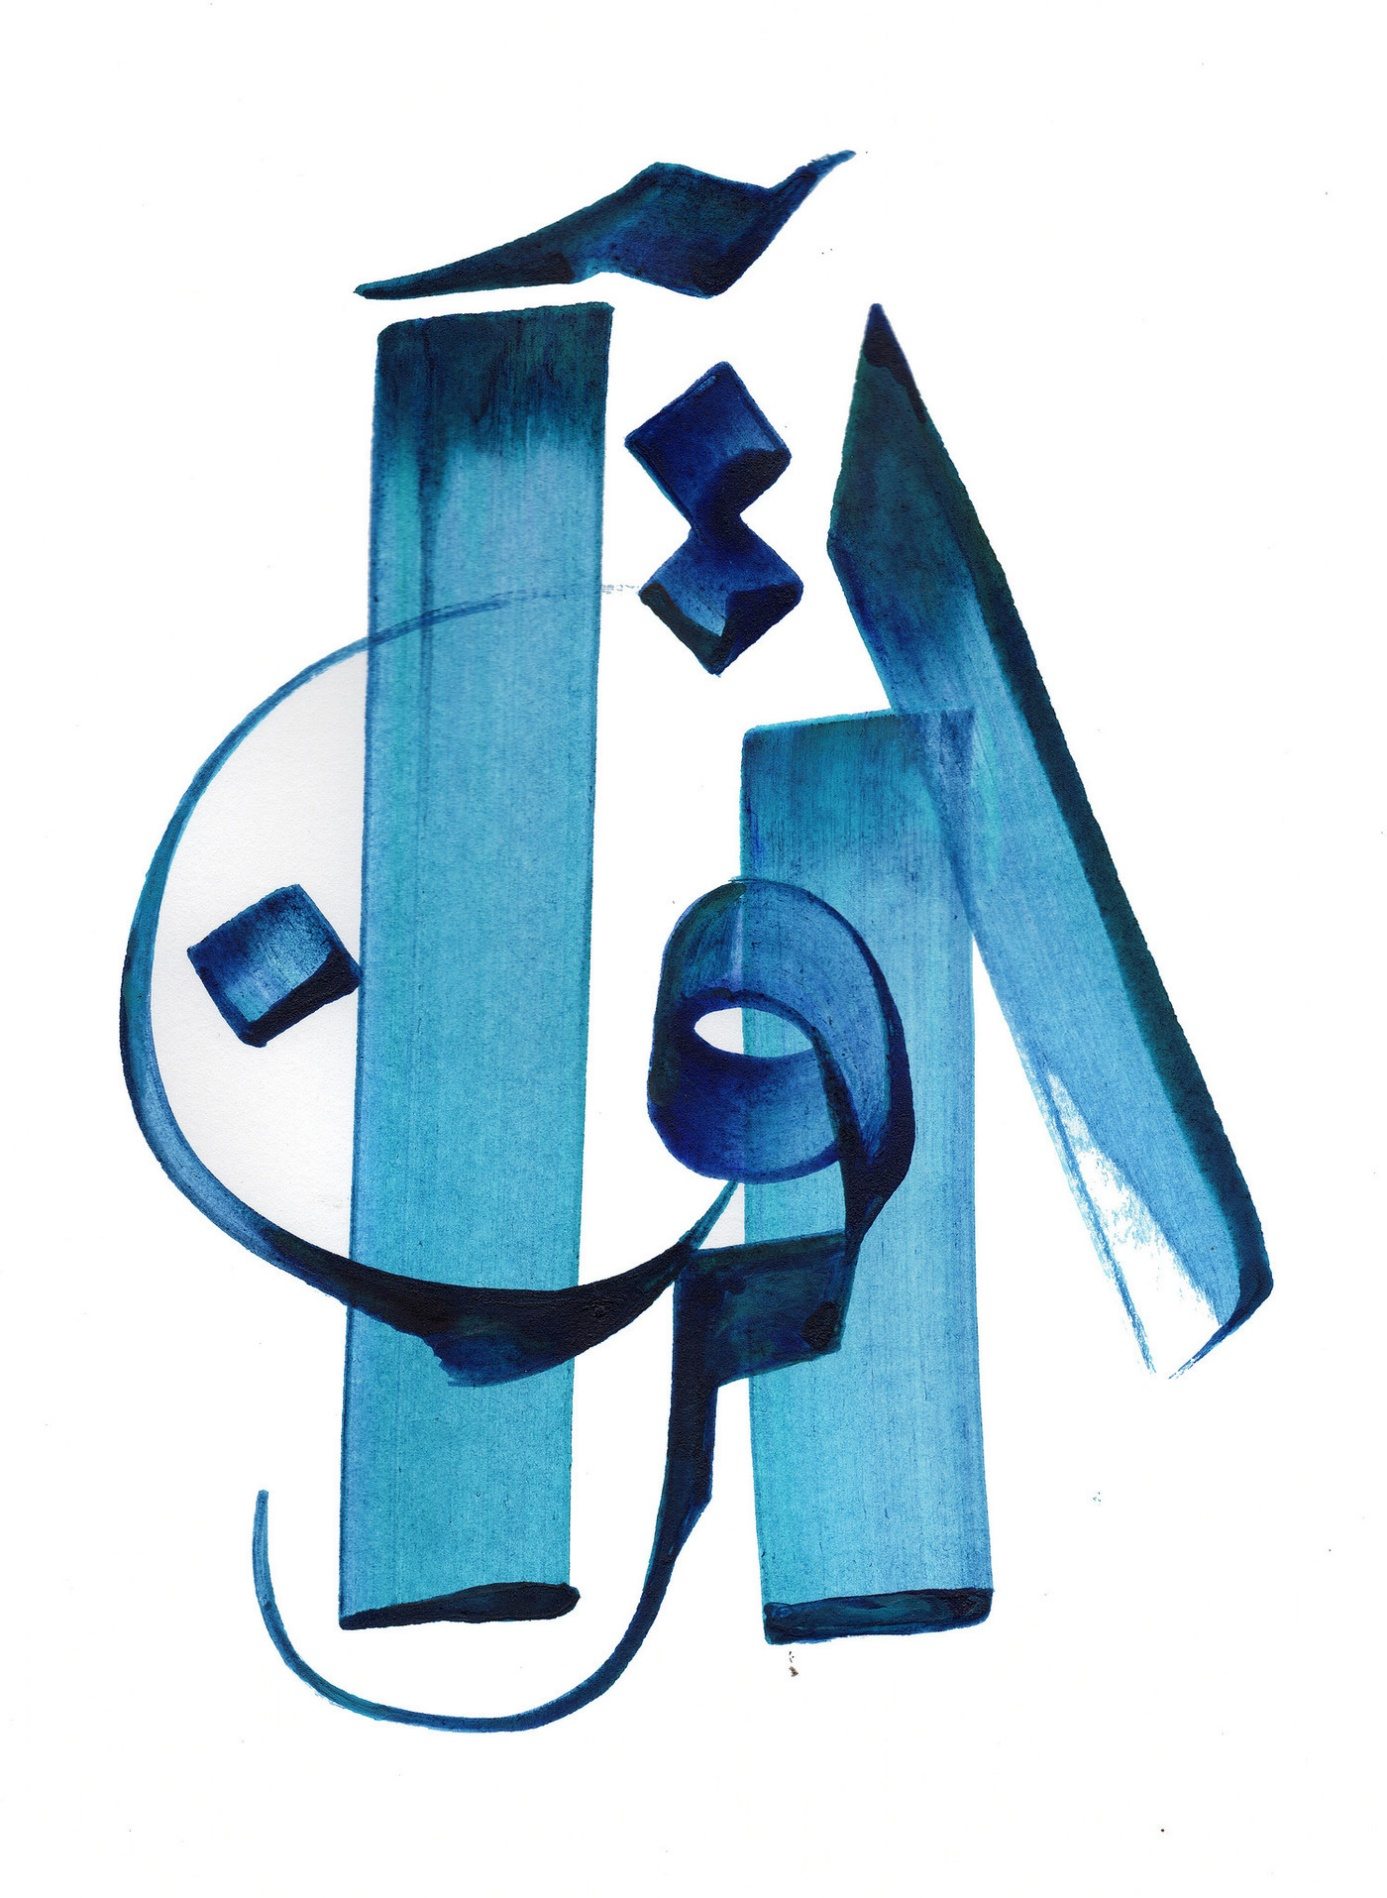
\includegraphics[width=\textwidth]{Images/image017.jpg}


\paragraph{Le regard de Hassan Massoudy}
\begin{cite}
« J'ai calligraphié le mot Coran autour de deux lignes droites,
verticales, qui forment comme l'architecture du mot. Elles lui donnent
une solidité. Avec ces deux axes, on se sent sécurisé. Ils supportent
tranquillement les autres lettres qui les chevauchent. Au centre de la
composition, une lettre forme comme un œil. Ici c'est la
lettre~\emph{qaf}-- pour le ``c'' de Coran --, qui est similaire à la
lettre~\emph{waw}. Lors d'un voyage en Turquie, j'ai découvert que les
soufis utilisaient la lettre~\emph{waw}~pour invoquer Dieu. C'est la
seule lettre de l'alphabet arabe qui, prise toute seule, peut signifier
quelque chose. Elle désigne donc l'Unique, mais sert aussi pour la
conjonction ``et''. Cette lettre évoque donc à la fois l'unique et le
multiple. »
\end{cite}


\vide{quest-ce-que-le-coran}{%
\section{{Qu'est-ce que le Coran~?
}{Qu'est-ce que le Coran~? }}\label{quest-ce-que-le-coran}}

Un livre~sacré ? Des prescriptions ? Des récits bibliques mais sans
ordre chronologique~? Que dit-il~? Comment est-il structuré~?

Avant d'exposer le Coran à la lumière de la foi musulmane, tel que les
théologiens, mystiques ou grands commentateurs l'ont compris, je vous
propose d'ouvrir quelques ouvrages récents écrits par des musulmans sur
le Coran. Ils donnent une première idée de ce que des musulmans disent
de lui et comment ils le voient.


\paragraph{Du côté des sheikh}
\mn{\textsc{Le Doute en Islam}. Le mot "islam" déjà, est l'antonyme même du doute. En effet, douter en Allah et en son Prophète est le reniement même de l'islam. Pourtant, dans la spiritualité musulmane, on peut parfois douter de soi-même et de sa capacité de croire et d'assimiler le bon et le vrai message. On peut aussi douter des interprétations et des constructions des uns et des autres mais jamais du Coran en tant que Parole révélée au Prophète. 
La seule école théologique qui, en terme de méthode, reconnaît que le "bon doute" pourrait contribuer au mûrissement de la foi, est celle rationaliste, le mo'tazilisme.  Grâce à l'esprit critique, les adeptes d'un tel courant exige de pratiquer le doute vis à vis des dogmes et des pratiques afin d'éviter tout assentiment aveugle et passif. 
Depuis Mohammad Arkoun (1928-2010) et ses héritiers, des exégètes et des historiens musulmans essaient en appliquant la méthode historico-critique  de "déconstruire" le dogmatisme régnant dans l'islam fondamentaliste.
}
\begin{Def}[Sheikh]
un sheikh, c'est un sage, un homme
doué de connaissances religieuses et scientifiques reconnues. En arabe,
cela veut dire maître,
vieillard.
\end{Def}
\label{un-sheik}
Le célèbre sheikh syrien \textbf{ʿAlī Ṭanṭāwī} \sn{voir p. \pageref{theo:AliAlTawani}}, (1909-1999) écrit dans
son livre \emph{Connaître l'islam} :
\mn{Tantâwî, \emph{Connaître l'islâm}.
  Citations respectives: p. 220, 241, 243, 242, cité par Anne-Sylvie
  Boisliveau, \emph{Le Coran par lui-même}, Brill, 2014.}.
  
  


\begin{quote}
    

«~Le musulman croit que le Coran est la parole de Dieu, apportée par
Gabriel à Muḥammad, qui l'a transmise comme il l'a entendue. Le musulman
ajoute foi que le contenu du Livre (Al-Mushâfe) dont nous disposons est
la totalité du Coran. Quiconque en nie une partie ou en doute sort de
l'Islâm.

Le Coran est le miracle de Muḥammad.

Le caractère inimitable du Coran est un fait, mais ne cherchez pas comme
les spécialistes de la rhétorique, les endroits inimitables du Coran. En
effet, ce qui est inimitable, ce ne sont pas seulement ses expressions,
ni son contenu métaphysique, mais sa globalité. Il est semblable à une
jolie femme. Sa beauté n'est pas dans la seule couleur de sa peau, dans
ses yeux, ou dans une seule partie d'elle, mais elle se trouve dans son
ensemble. Même si chaque observateur du Coran aperçoit le caractère
inimitable du côté qu'il observe.
 
{[}Muḥammad{]} a apporté un livre d'un style littéraire splendide ; au
sommet de la complétude en matière de droit ; en métaphysique il
contient des choses ignorées des hommes que la raison humaine ne peut
saisir d'elle-même~»
\end{quote}



\paragraph{Du côté des prédicateurs-missionnaires~:
}

Ahmad von Denffer (né en 1948), membre de la \emph{Fondation islamique}
et auteur d'un ouvrage sur les sciences coraniques, donne la définition
suivante~:
\begin{quote}
    

«~Le Coran contient les révélations d'Allāh, le Créateur et Maître de
l'Univers, à l'humanité~». Il est «~la parole d'Allāh, descendue sur le
dernier Prophète Muhammad par l'ange Gabriel, dans un sens et une
formulation précis, transmis par de nombreuses personnes (tawātur), à la
fois par oral et par écrit. Il est inimitable et unique, protégé par
Dieu de la corruption~»\mn{~Ahmad Von Denffer, \emph{`Ulūm
  al-Qur'ān. An Introduction to the Sciences of the Qur'ān}, The Islamic
  Foundation, 1988, p. 7~; 17.}.
\end{quote}
Harun Yahya (né en 1956), créationniste musulman, dans \emph{Des secrets
du Coran,} voit dans le Coran le livre qui contient toutes les vérités.
Il donne, dit-il, les secrets de l'humanité. Tous les résultats de la
science sont déjà inscrits dans le Coran, preuve de sa puissance. Il
écrit~en introduction~:
\begin{quote}
    

«~Le Coran fournit la connaissance véridique à l'homme et contient les
secrets de la création de Dieu dans sa forme la plus vraie et la plus
pure. Toute information non fondée sur le Coran et qui est en
contradiction avec ses versets est un leurre et une illusion. Par
conséquent, ceux qui n'adhèrent pas au Coran vivent dans un état
d'hallucination ici-bas et seront condamnés au châtiment éternel dans
l'au-delà. En dehors des prières, des ordres, des interdits et des
critères moraux élevés qui sont décrits dans le Coran, Dieu communique
beaucoup de secrets à l'humanité. Un œil attentif peut en témoigner
pendant toute sa vie~»\mn{Harun Yahya, \emph{Des secrets du
  Coran}, p. 9.}.
\end{quote}




\paragraph{Du côté des nouveaux penseurs~:
}

Ghaleb Bencheikh (né en 1960) dans son livre \emph{Le Coran} écrit~:
\begin{quote}
    

«~Formulé dans sa dimension la plus traditionnelle, le Coran est le
recueil des locutions divines révélées au prophète Muḥammad Ibn Abdallah
et transmises par l'ange Gabriel sur une période de vingt-trois années
lunaires~»
\end{quote}
Puis il ajoute~:
\begin{quote}
«~Plusieurs disciplines sont requises si l'on veut véritablement étudier
le Coran pour mieux l'appréhender, s'en emparer et en faire l'exégèse.
Différentes branches des sciences humaines et de l'étude des
civilisations concourent aux multiples axes autour desquels s'articule
la recherche herméneutique contemporaine. Elle s'appuie entre autres sur
la sémiotique, la médiologie la linguistique, la philologie, l'anagogie,
la paléographie et l'historiographie~»\mn{Ghaleb Bencheikh,
  \emph{Le Coran}, Paris, Eyrolles, 2010, p. 8-10.}.
\end{quote}
Ici, le philosophe souligne la nécessité d'intégrer le recours des
données des sciences humaines pour comprendre et interpréter le Coran.
Les seules sciences islamiques traditionnelles ne suffisent plus ou plus
exactement elles enferment le Coran dans une interprétation.

\paragraph{Mohammad Arkoun} (1928-2010) dans son ouvrage \emph{Lectures du
Coran}, note que


\mn{ Mohammed Arkoun (arabe \TArabe{ : محمد أركون, 1928} Algérie, mort en 2010 à
Paris, est un intellectuel algérien qui s'inscrit dans la tradition des
Lumières françaises, historien, islamologue et philosophe. Parmi ses
sujets de prédilection, l'impensé dans l'islam classique et
contemporain. humaniste, laïque, un militant actif du dialogue entre
les religions, les peuples et les hommes. Spécialiste de l'islam, il
plaidait pour un islam repensé dans le monde contemporain. Il y a
consacré de très nombreux ouvrages dont La Pensée arabe (Paris, 1975),
Lectures du Coran (Paris, 1982), Penser l'islam aujourd'hui (Alger,
1993)}
\begin{quote}
    

«~pour un esprit moderne habitué à suivre une démonstration, une
évocation, une description, un récit dans des textes composés selon un
plan rigoureux, le Coran est particulièrement rebutant par sa
présentation désordonnée, son usage inhabituel du discours, l'abondance
de ses allusions légendaires, historiques, géographiques, religieuses,
ses répétitions, ses inconséquences~»\mn{Mohammed Arkoun,
  \emph{Lectures du Coran}, Paris, Maisonneuve \& Larose, 1982, p. 1.}.
\end{quote}
Ces différents musulmans présentent d'une manière particulière le Coran,
donnant un éclairage singulier.
Bien que ces penseurs musulmans contemporains soient minoritaires, ils restent les pionniers de la production intellectuelle musulmane actuelle et l'actualisation de la doctrine islamique à la lumière des sciences humaines et sociales modernes. Même si une partie de l'imaginaire musulman actuel reste sous l'influence des écoles juridiques fondamentalistes, ces penseurs modernes sont très appréciés et écoutés par les musulman libéraux surtout ainsi qu'auprès des non-musulmans engagés dans le dialogue inter-religieux.   
Pour les plus intégristes, ils sont considérés comme \textit{zanadiqa}, hérétiques, blasphémateurs ou coupable d'apostasie. Et il ne faut pas oublier que, le blasphème est toujours puni de mort dans plusieurs islamiques.... En revanche, condamner à mort un penseur musulman reste un fait rare. Junaid Hafeez, par exemple, professeur d’université au Pakistan, était emprisonné depuis six ans quand il a été condamné à mort en décembre 2019 pour blasphème. Sa condamnation fait aujourd'hui l'objet d'un appel. A suivre ! Avec la prison, ils pourraient être interdits d'enseigner ou de se rendre dans des pays musulmans. On peut surtout aussi mettre sur l'Index leurs publications. L'Arabie Saoudite interdit l'ouvrage "Le Coran et ses lectures" d'Abdelmajid Charfi. 

Quoique dans le contexte actuel, l’islamisme considère que la critique du Prophète et sa représentation est l' acte le plus grave qui mérite le plus dur des châtiments, la critique de la Sunna pourrait être elle aussi compromise. Mais, il ne faut pas oublier, qu'actuellement en France, des penseurs musulmans contemporains qui n'hésitent pas de poursuivre leur méthode historico-critique. 

 Pour un premier approfondissement, il
convient de revenir à la méthode des savants de l'islam et de partir de
l'étymologie.

\vide{uxe9tymologie}{%
\subsection{Étymologie}\label{uxe9tymologie}}

La racine \emph{qara'a} signifie lire à haute voix, réciter. Par suite,
le \emph{Qur'ān} est une lecture. L'étymologie peut surprendre puisque
le \emph{Qur'ān}, avant d'être un livre, est donc une récitation d'un
livre. Pour les musulmans, cette récitation suscite une capacité
d'émotion religieuse bouleversante. Le Coran ne se lit pas, mais se
récite, se psalmodie. Il existe des règles précises et l'ensemble de ces
règles correspond au \emph{taǧwīd}. Le mot vient de la racine ǦaWaDa qui
signifie améliorer, rendre meilleur. On le distingue du \emph{tartīl}
qui est la lecture lente du Coran.

Les mosquées organisent parfois des concours de \emph{taǧwīd},
récitation du Coran, pour les enfants. C'est sur le principe de
\emph{The Voice}, avec un jury. Mais il note le participant en fonction
du respect des règles sur les pauses, les syllabes allongées, etc. Tout
y est beaucoup moins subjectif. Dans le film \emph{Wajda}, de 2012, qui
raconte avec beaucoup d'humour l'histoire d'une jeune enfant saoudienne
qui rêve d'avoir un vélo, on la voit dès les premières scènes du film
dans une école coranique où elle apprend le Coran. L'apprentissage du
Coran n'est pas réservé aux seuls hommes~! Pour autant, le film est très
ironique car en déplaçant bien des problématiques d'adultes dans le
monde de l'enfance, il n'en dessine pas moins un triste tableau de la
condition des femmes en Arabie. A son camarade, Wajda dit qu'elle veut
faire du vélo avec lui, mais lui de lui répondre~: «~ce n'est pas
possible, tu es une femme~». Et elle de renchérir~: «~tu dis ça, parce
que tu sais que si je faisais du vélo je serai meilleure que toi~».

\vide{section-13}{%
\subsubsection{}\label{section-13}}

\vide{extrait-de-la-ruxe9citation-coranique-par-un-iranien-de-7-ans-devant-un-public-manifestement-conquis-uxe9coutez-jusquuxe0-la-fin.}{%
\subsubsection{{Extrait de la récitation coranique par un
iranien de 7 ans devant un public manifestement conquis\ldots{} écoutez
jusqu'à la fin.
}{Extrait de la récitation coranique par un iranien de 7 ans devant un public manifestement conquis\ldots{} écoutez jusqu'à la fin. }}\label{extrait-de-la-ruxe9citation-coranique-par-un-iranien-de-7-ans-devant-un-public-manifestement-conquis-uxe9coutez-jusquuxe0-la-fin.}}

Cette puissance affective ou émotionnelle de la récitation coranique est
affirmée par le Coran lui-même~:
\begin{quote}
    
«~Il dit de lui-même que cette lecture est splendide~: «~Dis~:
`croyez-le ou ne le croyez pas, à ceux à qui le savoir a été donné avant
cela, lorsque l'on leur récite {[}le Coran{]}, ils tombent prosternés
sur leurs faces~» (S. 17, 107).

\TArabe{قُلْ آَمِنُوا بِهِ أَوْ لَا تُؤْمِنُوا إِنَّ الَّذِينَ أُوتُوا
الْعِلْمَ مِنْ قَبْلِهِ إِذَا يُتْلَى عَلَيْهِمْ يَخِرُّونَ
لِلْأَذْقَانِ سُجَّدًا}

\end{quote}

Mais avant de poursuivre sur la manière dont le Coran parle de lui-même,
il importe de décrire le livre, de découvrir sa structure, sa
composition.

\vide{composition-et-structure-du-coran}{%
\section{1.~Composition et structure du
Coran}\label{composition-et-structure-du-coran}}

\vide{un-livre-formuxe9-de-sourates}{%
\subsection{{1.1 Un livre formé de sourates
}{1.1 Un livre formé de sourates }}\label{un-livre-formuxe9-de-sourates}}

\vide{terminologie-et-nombre-des-sourates}{%
\subsubsection{1.1.1 Terminologie et nombre des
sourates}\label{terminologie-et-nombre-des-sourates}}

Le Coran est composé de 114 sourates, ordonnées de la plus longue à la
plus courte -- comme pour les épîtres de Paul -- à l'exception de la
première qui s'apparente à une prière introductive. Nous reviendrons sur
cette première sourate qui s'apparente très étrangement au Psaume
1\textsuperscript{er}. L'ouverture du Coran, comme l'ouverture du
Psautier~? C'est bien ce que je dis. Et une analyse intertextuelle le
prouve. Ouvrez l'un et l'autre et regardez, comparez.
\mn{Comparaison entre le Ps 1 et la sourate \textit{Al-Fatiha (L'ouverture)}}
\begin{longtable}{p{4.2cm}p{4.2cm}p{3cm}}
\toprule
Ps 1 & Al-Fatiha (L'ouverture) &\TArabe{ سورة الفاتحة }\\
\midrule
\endhead
& Au nom d'Allah, le Tout Miséricordieux, le Très Miséricordieux.

Louange à Allah, Seigneur de l'univers.

Le Tout Miséricordieux, le Très Miséricordieux, &\TArabe{ بِسْمِ اللَّهِ
الرَّحْمَنِ الرَّحِيمِ

2 الْحَمْدُ لِلَّهِ رَبِّ الْعَالَمِينَ

3 الرَّحْمَنِ الرَّحِيمِ }\\
{1. Heureux l'homme qui ne marche pas selon le conseil des
méchants, Qui ne s'arrête pas sur la voie des pécheurs, Et qui ne
s'assied pas en compagnie des moqueurs,} & & \\
{2. Mais qui trouve son plaisir dans la loi de l'Eternel, Et qui la
médite jour et nuit!} & & \\
{3. Il est comme un arbre planté près d'un courant d'eau, Qui donne
son fruit en sa saison, Et dont le feuillage ne se flétrit point: Tout
ce qu'il fait lui réussit.} & & \\
{4. Il n'en est pas ainsi des méchants: Ils sont comme la paille
que le vent dissipe.} & & \\
{5. C'est pourquoi les méchants ne résistent pas au} jour du
jugement\textbf{, Ni les pécheurs dans l'assemblée des justes;} &
4.Maître du \textbf{Jour de la rétribution.}

C'est Toi {[}Seul{]} que nous adorons, et c'est Toi {[}Seul{]} dont nous
implorons secours. &\TArabe{ 4 مَالِكِ يَوْمِ الدِّينِ

5 إِيَّاكَ نَعْبُدُ وَإِيَّاكَ نَسْتَعِينُ }\\
{6. Car l'Eternel connaît la} voie des justes\textbf{, Et la voie
des} pécheurs mène à la ruine\textbf{.} & Guide-nous dans le
\textbf{droit chemin,}

\textbf{le chemin de ceux que Tu as comblés de faveurs}, non pas de ceux
qui ont encouru Ta colère, ni \textbf{des égarés}. &\TArabe{ 6 اهْدِنَا
الصِّرَاطَ الْمُسْتَقِيمَ

7 صِرَاطَ الَّذِينَ أَنْعَمْتَ عَلَيْهِمْ غَيْرِ الْمَغْضُوبِ عَلَيْهِمْ
وَلَا الضَّالِّينَ }\\
\bottomrule

\end{longtable}

\begin{Def}[āyat]
Chaque sourate (\emph{sūra}) est composée de versets (\emph{āyah},
\emph{āyat}) mot qui signifie au préalable signe~: chaque verset est en
lui-même un signe donné par Dieu
\end{Def}


\vide{on-retrouve-ce-mot-dans-ayatollah-qui-veut-donc-dire-signe-de-dieu}{%
\mn{on retrouve ce mot dans ayatollah, qui veut donc
dire~\ldots{} signe de
dieu}\label{on-retrouve-ce-mot-dans-ayatollah-qui-veut-donc-dire-signe-de-dieu}}

 Selon les lexicographes, \emph{āyah} renvoie à l'idée de merveille, de
prodige. Le mot souligne la dimension prophétique et prodigieuse du
signe transmis à Muḥammad.

Le terme de sourate (\emph{sūrat}) apparaît à neuf reprises dans le
coran au singulier et une fois au pluriel. Sa signification reste
confuse. Les lexicographes remarquent qu'il provient de la racine SWR
qui signifie monter sur un mur, se hisser sur, assaillir, fondre sur
quelqu'un, être impétueux\sn{~\textsc{Gloton}, \emph{Lexique},
  n°0756, p. 466. Voir aussi Roger \textsc{Arnaldez}, \emph{Le Coran,
  Guide de lecture}, Paris, Desclée, 1983, p. 36.}. \emph{Sūrat}
signifie à la fois rangée de pierre, trace, indication, signe. Chez le
commentateur \textbf{Faḫr al-Dīn al-Rāzī}.


{c'est encore un nom nouveau, mais on ne peut parler du
Coran sans très vite parler d'al-Rāzī. Il est en effet l'auteur d'un des
plus sublimes commentaires du Coran, \emph{Les clefs de l'invisible}.C'est un Persan du XII\textsuperscript{e} siècle.}
\sn{Michel Lagarde
  a consacré une belle étude sur ce Commentaire~: Michel
  \textsc{Lagarde}, \emph{Les secrets de l'invisible : Essai sur le
  Grand Commentaire de Fahr al-Dîn al-Râzî}, Paris, Albouraq, 2009.}. 

on trouve l'idée selon laquelle de même qu'une muraille entoure une
ville de tout ce qu'elle contient, de même la \textbf{sourate enveloppe
la science contenue dans le Coran}. L'idée de mur ou de muraille est
aussi interprétée comme signifiant l'élévation du croyant qui
s'approprie l'enseignement du Coran~: c'est l'interprétation donnée par
\textbf{Qurṭubī} (1214-1273), autre grand exégète du Coran.

Mais pourquoi y a-t-il des sourates~? Pourquoi le Coran n'est-il pas
écrit en un seul bloc~? Pourquoi donc une composition~de plusieurs
éléments ? Cette question est typique de celles que l'on trouve dans le
commentaire de \textbf{Faḫr al-Dīn al-Rāzī} où il se demande
systématiquement pourquoi les choses sont ainsi et pas autrement~:
pourquoi telle construction grammaticale, pourquoi tel mot sous telle
forme, pourquoi tel ordre et ici, pourquoi des sourates et pas tout
simplement un Livre en un seul tout\textbf{.} \mn{Roger Arnaldez expose la
réponse d'al-Rāzī dans son livre \emph{Le Coran Guide de lecture}.}

\vide{nom-des-sourates}{%
\subsubsection{{Nom des sourates
}}\label{nom-des-sourates}}

Chaque sourate est désignée par un nom. Cette désignation semble tardive
puisque les compagnons de Muḥammad à La Mecque rapportent des versets
des sourates à partir de leurs noms. Le nom des sourates dépend d'un
thème ou d'un élément cité dans la sourate. Ainsi, par exemple, la
sourate al-Tawba porte sur le repentir accueilli par Dieu à Muḥammad, à
ceux qui étaient avec lui et à ceux qui étaient restés derrière lui. Il
y a quelques étrangetés, comme le nom de la Sourate
2\textsuperscript{e}, la Vache, \emph{al-Baqara}. Le thème est tiré des
Nombres et du Deutéronome en lien avec Moïse. Or, l'épisode de la vache
ne couvre que huit versets sur 286 (versets 67-73).

\vide{nature-des-sourates}{%
\subsubsection{Nature des sourates}\label{nature-des-sourates}}

Certaines sourates sont très particulières : la première sourate par
exemple, al-Fātiḥa, l'Ouvrante, est une prière adressée à Dieu par les
croyants. Elle illustre parfaitement l'élaboration progressive du texte
coranique : on en a trouvé des variantes textuelles dans des traditions
ou des ouvrages anciens. Une teneur identique, mais des mots, des
constructions syntaxiques différentes.

La sourate 111 (\emph{al-masad}, la corde) est une formule de
malédiction de type archaïque. Rien dans le texte ne spécifie ce dont il
s'agit. Il est donc une énigme. Les circonstances de la Révélation
diront plus tard qu'il s'agit d'une malédiction prononcée par Muhammad
contre un de ses oncles hostile à sa prédication. Nous avons déjà
rencontré son nom. Ce serait Abū Lahab.

Les deux dernières sourates sont des incantations magico-prophylactiques
(pour préserver la santé). Elles semblent avoir suscité bien des litiges
quant à leur insertion.

Le Coran comporte des proclamations oraculaires (comme les oracles qui
rapportent ce qu'ils voient), des hymnes sous une forme poétique :
l'évocation poétique du Paradis est une adaptation arabe originale des
Hymnes d'Ephrem de Nisibie, Père de l'Église syriaque (+ 373). Oui, les
versets eschatologiques sur les houris sont des échos des hymnes de St
Ephrem. Sur ce point, les travaux d'intertextualité d'Andrae Tor sont
une référence incontournable et plus récemment de Christoph
Luemberg\sn{Tor Andrae, \emph{Les origines de l'islam et le
  christianisme}, Paris, 1955.
\sn{
   le compte-rendu de ce livre dans la Revue d'histoire des
  religions
  \url{http://www.persee.fr/doc/rhr\_0035-1423\_1957\_num\_151\_2\_8712}.}.}

Il y a des récits, des textes législatifs et parénétiques (exhortatifs).
On y trouve aussi des discours de guerre, d'appel au combat
(\emph{ğihād} ou \emph{qitāl})\sn{Emmanuel \textsc{Pisani}, «~La
  violence dans le Coran~», sur le site~:
  \url{http://www.croire.com}{www.croire.com} , juin 2015.}. Cette
guerre est contre plusieurs ennemis : les gens du Livre qui ne
pratiquent pas la religion de la vérité (S. 9, 111).

Il y a aussi des discours polémiques~: Mehdi Azaiez, - il a consacré sa
thèse de doctorat à l'analyse de ce genre littéraire dans le Coran -,
remarque qu'il s'agit de «~l'un des genres les plus marquants du corpus
coranique~»\sn{Medhi \textsc{Azaiez}, «~Le contre-discours
  coranique. Premières approches d'un corpus~», dans Azaiez,
  \emph{Nouvelles approches du} Coran, Paris, CNRS, 2013, p 257.}. On
trouve ainsi cette invitation à «~débattre de la meilleure
façon~»~(S.16, 125)\sn{~Jane Dammen \textsc{McAuliffe}, «~Debate
  with them in a better Way : the Construction of a Qur'anic
  Commonplace~», dans \emph{Myths, historical archetypes and symbolic
  figures in Arabic literature towards a new hermeneutic approach},
  Proceedings of the International Symposium in Beirut, June 25th-June
  30th, 1996, / Edited by Angelika Neuwirth, Birgit Embaló, Sebastian
  Günther, 1999, p. 163-188.} :
\begin{quote}
    
«~Appelle les hommes dans le chemin de ton Seigneur par la sagesse et
une belle exhortation~; discute avec eux de la meilleure manière~»

\TArabe{ادْعُ إِلَى سَبِيلِ رَبِّكَ بِالْحِكْمَةِ وَالْمَوْعِظَةِ
الْحَسَنَةِ وَجَادِلْهُمْ بِالَّتِي هِيَ أَحْسَنُ إِنَّ رَبَّكَ هُوَ
أَعْلَمُ بِمَنْ ضَلَّ عَنْ سَبِيلِهِ وَهُوَ أَعْلَمُ بِالْمُهْتَدِينَ}
\end{quote}

Il fait remarquer que la polémique est inhérente à l'islam originel dans
la mesure où la parole de Muḥammad a d'abord été rejetée par le groupe
tribal auquel il appartenait. C'est donc avec les siens qu'il a fallu
d'abord débattre et convaincre si bien que la question de la polémique
émerge dès la naissance de l'islam. Les débats, les réponses formulées
aux contradictions sont inhérents au texte et peuvent se traduire par
des incantations, des malédictions, des reproches, des avertissements,
des railleries, des apostrophes en direction des
non-croyants\sn{Neal \textsc{Robinson}, \emph{Discovering the
  Qur'an}, p. 116, cité par Azaiez, \emph{op. cit}., p. 259.}.

\vide{agencement-des-sourates}{%
\subsubsection{{Agencement des sourates
}}\label{agencement-des-sourates}}

Autre question, celle de l'agencement des sourates et l'ordre des
versets. Quel ordre suivre~? Cette question est au cœur d'une
\emph{disputatio} entre les savants musulmans.

L'exégète al-Qurṭubī (nous avons déjà rencontré ce noms avec al-Rāzī)
rapporte les propos du Qāḍī Abū Bakr Ibn Al-Ṭayyib~: «~On peut faire
l'objection que les Anciens ont été en désaccord sur l'ordre des
sourates du Coran. Certains, dans leur recueil, ont écrit les sourates
selon la chronologie de leur révélation, et ils ont mis en tête les
sourates mecquoises, puis les sourates médinoises~; certains commencent
par la louange al-Ḥamd, d'autres par la sourate 96~: `Récite, au nom de
ton Seigneur qui créa\ldots'~: tel est le début du recueil de `Alī.
Quant à celui d'Ibn Mas`ūd, il commence par `Maître du Jour du Jugement
(1,3), puis viennent la sourate \emph{La Vache} (2) et la sourate
\emph{Les femmes} (4)\ldots{} Le recueil d'Ubayy débute par al-Ḥamd~;
suivent les sourates 3, La Famille de `Imrān la sourate 6, les
Troupeaux, la sourate 7, al-`Araf, la sourate 5, La Table et ainsi de
suite\ldots{} avec de profondes divergences~»\sn{Cité par
  \textsc{Arnaldez}, \emph{Le Coran. Guide de lecture}, \emph{op. cit}.,
  p. 47.}.

L'exégète ici se fait l'écho d'un débat quant à l'agencement des
sourates au sein même de la tradition musulmane. La découverte d'anciens
manuscrits du Coran à San`ā au Yémen, en 1972 confirme l'existence de
différents corpus coraniques. Muḥammad Amir Moezzi écrit~à ce propos~:
«~En sus de quelques variantes orthographiques et lexicographiques
mineures, 22\% des 926 groupes de fragments étudiés présentent un ordre
de succession de sourates complètement différent de l'ordre connu~: le
découpage en versets ne correspond à aucun des 21 systèmes connus. Ce
qui est frappant c'est que l'ordre des sourates se rapproche le plus des
codex d'Ubbay et d'Ibn Mas`ūd~»\sn{\textsc{Cuypers, Gobillot},
  \emph{Idées reçues}, p. 18.}.

Il semble donc qu'existèrent entre ces recensions des différences, à la
fois dans l'ordre, mais aussi dans le texte. Mais retenez aussi que la
tradition musulmane rapporte l'existence de différents corpus~: elle les
canonise d'une certaine façon. Parmi ces corpus, la tradition sunnite
reconnaît que `Alī avait élaboré son corpus\ldots{} Corpus dans lequel
serait inscrit, d'après la tradition šī`ite, les versets divins qui
désignaient `Alī comme successeur de Muḥammad\ldots{}

\vide{un-livre-en-arabe-clair}{%
\subsection{1.2 Un livre en arabe clair}\label{un-livre-en-arabe-clair}}

«~Voici un Livre dont les versets sont clairement exposés~; un Coran
arabe, destiné à un peuple qui comprend~» (S.~41, 2-3).

Et le Coran de préciser «~un arabe clair (\emph{`arabiyyun mubīn})~» (S.
16, 103 et 26, 195).

Le Coran de lui-même accorde une importance singulière à la langue
arabe. On comprend pourquoi, face à une question, il convient de revenir
aux mots arabes et à leur signification.

L'arabe est comme magnifié. Mais cet arabe est-il si clair~comme
l'affirme le Coran ? Et s'il l'est, pourquoi tant de niveaux de
commentaires, et d'explications parfois contradictoires~? Pourquoi le
prophète Muḥammad a-t-il dû expliquer les significations du Coran à ses
compagnons~? Quel crédit et quelle autorité accorder aux explications
propres aux compagnons~eux-mêmes ? Ces questions nous introduisent dans
une des difficultés propres à tout texte sacré et qui est sa
compréhension. Comme le dit Tariq Oubrou, imam de Bordeaux, «~il ne
suffit pas de lire le Coran pour le comprendre~».

\vide{histoire-du-coran-sa-constitution-muux1e63ux1e25af}{%
\section{{2. Histoire du Coran~: sa constitution
(\emph{muṣḥaf}
)}{2. Histoire du Coran~: sa constitution (muṣḥaf )}}\label{histoire-du-coran-sa-constitution-muux1e63ux1e25af}}

Depuis quand le Coran existe-t-il sous la forme qui est la sienne
aujourd'hui~? Muḥammad a-t-il eu de son vivant et sous ses yeux le texte
coranique tel qu'il est structuré~? Il n'en est rien et la constitution
du \emph{muṣḥaf}, c'est-à-dire le Coran dans sa matérialité, n'est pas
effective avant la fin du premier siècle de l'Hégire. Elle souligne que
l'islam s'inscrit pleinement dans la tradition de l'oralité, et avant
d'être un livre, le Coran était une récitation. Mais pourquoi a-t-on
éprouvé le besoin de rassembler les sourates en un livre~? Tel est
l'objet de la présente partie.

\vide{linitiative-dabux16b-bakr}{%
\subsection{{2.1 L'initiative d'Abū Bakr
}{2.1 L'initiative d'Abū Bakr }}\label{linitiative-dabux16b-bakr}}

Selon la tradition, à la mort de Muḥammad, en 632, la Révélation est
connue par cœur et dans son intégralité par quelques rares fidèles qui
sont appelés les lecteurs du Coran (\emph{qurrā'} -- on retrouve la
racine QR' comme dans \emph{Qur'ān}, Coran). Leurs noms divergent selon
les traditions. Mais le Coran comme \emph{muṣḥaf} n'existe pas encore.

À la mort de Muḥammad, Musaylima, celui qui se prétendait aussi prophète
et qui a écrit une lettre à Muḥammad -- épisode de la Sīra que nous
avons rencontré dans le précédent chapitre -- jouissait d'une certaine
aura. Le voici qui vient trouver Abū Bakr, le premier successeur de
Muḥammad, le premier calife donc, et affirme : «~Gabriel est venu me
trouver et m'a confié la mission de prophète par toute la terre~». Il
s'insurge contre le calife et met en déroute le premier général envoyé.
En l'année 633, Abū Bakr charge Ḫālid Ibn al-Walīd de mettre un terme
aux agissements de Musaylima. C'est la bataille de `Aqrabā. Il y trouva
la mort.

Cependant, au cours de la bataille, de nombreux récitants
(\emph{qurrā'}) trouvèrent aussi la mort. `Umar aurait pris conscience
du risque de perdre des fragments du Coran. Il en informe le calife Abū
Bakr qui charge Zayd Ibn Thabit de rassembler les sourates sur des
feuilles. La tradition est rapportée ainsi par Buḫarī dans la
\emph{Sunna}, au Livre 66, chapitre 3.

«~Zayd ibn Ṯābit a dit~: «~Abū Bakr vint me faire chercher à la suite du
massacre des gens de Yamāma. Lors {[}de ma venue{]} je trouvai Abū Bakr
chez lui et il me dit~: `Umar vient de m'informer que le massacre qui
eut lieu à Yamama a mis fin à la vie de lecteurs du Coran et je crains
que si le combat devait perdurer, ils continuent de se faire tuer sur
les champs de bataille, si bien que disparaîtrait une bonne partie du
Coran. C'est pourquoi je pense qu'il te faut collectionner le Coran'\,'.
J'ai alors dit à `Umar : `Comment vas-tu faire quelque chose que le
Messager d'Allah n'a pas faite~?'\,' -- `Umar dit~: Par Allāh,~ceci est
une bonne chose ». Il ne cessa de me répéter son idée jusqu'à ce
qu'Allāh m'ouvrit le cœur et me fit adhérer à ce qu'\,`Umar avait
proposé.~»

Zayd dit~alors qu'Abū Bakr avait poursuivi en disant~: `tu es un homme
jeune, raisonnable et au-dessus de tout soupçon et tu transcrivais déjà
par écrit la révélation pour le prophète. Collecte et rassemble donc le
Coran'. Par Dieu, me disais-je, s'il m'avait mandaté pour déplacer une
montagne, cela m'aurait été plus aisé que d'exécuter l'ordre de
rassembler le Coran. Je dis : `comment allez-vous faire quelque chose
que le Messager d'Allah n'a pas faite~? Mais il (Abū Bakr) dit~: «~Par
Allāh, c'est une bonne chose.~» Et puis il ne cessa de me répéter son
idée jusqu'à ce qu'Allāh m'en inspirât l'admission comme Il l'avait fait
pour Abū Bakr et pour `Umar. Dès lors, je me suis mis à rechercher et à
collecter les éléments coraniques transcrits sur des branches de dattier
et sur des pierres lisses ou conservées dans la mémoire des gens et j'ai
trouvé les derniers versets de la sourate \emph{at-Tawba} chez Abū
Ḫuzayma al-Anṣārī que je n'avais pas trouvés chez les autres\ldots{} Les
feuilles contenant le Coran furent conservées par Abū Bakr jusqu'à sa
mort puis elles furent déposées auprès d'\,`Umar qui les garda jusqu'à
sa mort puis elles furent transférées à sa fille Ḥafṣa.

De cette tradition, on peut retenir avec une certaine assurance qu'une
compilation fut entreprise à l'époque d'Abû Bakr. `Umar les accueillit
puis sa fille, Ḥafṣa.


\mn{ Vous avez lu que je vous ai parlé de la
bataille de `Aqarbā, mais la tradition parle des gens de Yamāma\ldots{}
alors~? En fait, `Aqrabā est le nom d'une plaine de la région de Yamāma.
J'ajouterai aussi que d'après la tradition musulmane, Abū Bakr avait
envoyé 3000 hommes~! Ce qui veut dire aussi que Musaylima avait des
disciples et nombreux étaient aussi ceux qui suivaient ses prophéties.
La région semble connaître un embrasement prophétique. a bataille
d'Al-Yamama (arabe \TArabe{
اليمامة} 
)
ou bataille d'al-`Aqrabā aura eu lieu, selon
les sources musulmanes, en 633, dans le cadre des Guerres de Ridda
(l'Apostasie), sur la plaine de Aqraba dans la région d'Al-Yamama (dans
l'actuelle Arabie Saoudite) entre les forces du calife Abou Bakr le
véridique et Musaylima le menteur, un prophète autoproclamé.
}


\subsection{{La constitution de la Vulgate de `Uṯmān
}}\label{la-constitution-de-la-vulgate-de-uux1e6fmux101n}

C'est donc sous `Uṯmān (l'impulsion vient d'Abū Bakr, mais la
constitution lui est postérieure~: il ne vécut pas assez longtemps) que
l'on entreprit la collection du Coran. Outre le récit transmis par la
tradition, l'histoire montre que cet acte est loin d'être purement et
simplement religieux. Il revêt une dimension politique~: il s'agit de
\textbf{contrebalancer le pouvoir des lecteurs qui se sont institués
gardiens du texte sacré}. Cela sert par ailleurs la politique
centralisatrice déployée par le troisième calife.

Mais si l'initiative califale permet au calife de concentrer les
pouvoirs politiques et religieux, il n'est pas le seul à vouloir
constituer une Vulgate.

\vide{la-constitution-dautres-corpus}{%
\subsection{{2.3 La constitution d'autres corpus
}{2.3 La constitution d'autres corpus }}\label{la-constitution-dautres-corpus}}

Ainsi, certains compagnons du Prophète, attachés à la transmission de la
Parole, vont proposer leurs propres recensions. On a ainsi parlé d'un
corpus de Sālim Ibn Ma`qil -- mais il est mort un an après le Prophète.
Plus solide, serait la recension d'un cousin de Muḥammad, `Abd Allāh Ibn
`Abbās (m. 68 / 688). Ce corpus est aujourd'hui perdu.

\mn{{`Alī} -- petit rappel~: c'est le cousin et le gendre de
Muḥammad, le premier converti à l'islam selon la \emph{Sīra} --, selon
les šī`ites, était aussi en sa possession du \emph{muṣḥaf}.}

On trouve aussi le corpus d'Abd Allāh \textbf{Ibn Mas`ūd} (m. 30 / 650),
un des premiers convertis à l'islam, très proche du Prophète. Lui aussi
va rédiger un corpus. On sait à partir de citations diverses dans des
ouvrages anciens que différentes recensions circulaient. La version
d'Ibn Mas`ūd a par exemple circulé à Koufa en Irak puisque le gouverneur
d'Irak exigea de détruire ce corpus. Or, en 1007, le même ordre fut
répété à Bagdad ce qui signifie bien qu'il n'avait pas été complètement
détruit. Cela indique aussi qu'il présentait des divergences par rapport
à la Vulgate de `Uṯmān.

Toutefois, les variantes entre les différents codex semblent avoir été
minimes. On a établi que la version de Mas`ūd ne comportait pas la
première sourate, ni les deux demandes de protections (S. 113 et 114).
On a émis l'hypothèque très plausible que ces trois sourates formaient
un encadrement liturgique qui apparemment n'étaient pas dans le Coran
primitif. Vous vous souvenez du Psaume 1 qui ouvre le Psautier\ldots{}

Dès le premier siècle, un autre débat voit le jour quant à la manière de
réciter le Coran et à la nature même des consonnes qui sont utilisées.
On a un écho de cette question dans la Sunna. En effet, certains
lecteurs lisaient en recourant à d'autres lettres ce qui entraina des
divergences de lectures. Elles étaient nombreuses entre l'Irak et en
Syrie et ils s'en suivaient des accusations d'anathèmes réciproques. Il
faut bien voir que l'écriture arabe présentait des déficiences puisque
des phonèmes différents comme b, t, ṯ, n, y, étaient écrits avec le même
signe alphabétique. De plus, les signes indiquant les voyelles n'étaient
pas inscrits ce qui orientait le texte dans des sens grammaticaux
pluriels. Par conséquent, il y avait des traditions de lectures
(\emph{qirā'āt}) différentes selon les villes et les régions. Avec les
conquêtes, l'islam était prêché dans des contrées où existaient d'autres
dialectes et surtout d'autres prononciations. Un Égyptien ne prononce
pas la lettre \emph{dji}, mais il dit \emph{gué} -- ce que ne fait pas
le Syrien. Demandez à un Arabe de prononcer la lettre p\ldots{} il ne
dira pas \emph{p}ardon, mais \emph{b}ardon.

C'est dans ce contexte que l'on a renvoyé à un \emph{ḥadīṯ} sur les
lectures du Coran. Ainsi, on trouve dans la Sunna
d'\textbf{al-Buḫarī}~-- c'est un des très grands compilateurs de l'islam
de ḥadīṯ. Son nom sera revu et revu dans le prochain chapitre.


\subsubsection{Ces 5 variantes de Harf sont un moyen de rentrer dans une
pluralité de
sens}
\begin{quote}
    «~Un jour, lors du vivant du Prophète, j'entendis Hishâm ibn Hakîm
réciter la sourate al-Furqân. Alors que j'écoutais avec attention sa
récitation, je m'aperçus qu'il recourait à certaines lettres différentes
de celles que le Prophète m'avait enseignées. Je m'apprêtais à
l'interpeller durant sa prière, mais je me retins et attendis qu'il la
terminât. Je le pris alors par son vêtement et lui dis : "Qui donc t'a
enseigné ainsi la sourate que je t'ai entendue réciter ? -- C'est le
Prophète, me répondit-il. - Tu mens, lui répliquai-je, car il me l'a
enseignée avec des lettres différentes que certaines de celles que tu
viens de réciter." Je l'emmenai alors auprès du Prophète et exposai à
celui-ci le problème : "J'ai entendu cet homme réciter la sourate
al-Furqân avec certaines lettres autres que celles que tu m'as
enseignées. -- `Laisse-le' me dit le Prophète. Puis, se tournant vers
Hishâm, il lui dit : "Récite, Hishâm." Hishâm récita alors la sourate de
la même manière qu'il l'avait faite auparavant. Le Prophète dit alors :
`Ainsi a été révélée cette sourate'. Puis il me dit : `Récite, toi,
Umar'. Je le fis alors selon la façon que lui-même m'avait enseignée. Il
dit également : `Ainsi a été révélée cette sourate'. Puis il conclut :
`Le Coran est révélé selon sept variantes de récitation (\emph{harf}).
Récitez donc celle qui est facile pour vous'\emph{~(rapporté par
al-Bukhârî, Ṣaḥih ~Book 97, Hadith 175, n° 4706)}~»\emph{.}
\end{quote}


Vous ne le saviez peut-être pas, mais il y a donc plusieurs manières de
lire le Coran, avec d'autres consonnes, et donc d'autres mots, et donc
d'autres significations. Ce \emph{ḥadīṯ} permet de mettre fin à des
divergences de lectures qui devaient être conflictuelles et de
réconcilier ainsi tous les musulmans. À l'intérieur même du texte,
l'uniformité de lecture n'est donc pas absolue. Peu à peu s'imposèrent
des versions majoritaires, au X\textsuperscript{e} siècle, et on limita
les lectures à 7, 10 et 14 versions différentes.

La constitution officielle du Coran impulsée par `Uthman, trouve son
achèvement sous le règne de `Abd al-Malik (m. 705). Elle a été largement
combattue par les milieux šī`ites qui y ont vu une tentative d'imposer
une version falsifiée du Coran. En effet, pour les šī`ites, la version
en possession de `Alī indiquait des prérogatives particulières accordées
à `Alī et sa famille. Notamment, Dieu aurait révélé le nom du successeur
de Muḥammad, qui n'était autre que\ldots{} `Alī. On en a une
illustration dans le \emph{Kitāb al-Qirā'āt} ou \emph{al-Tanzīl wa
l-taḥrīf} d'al-Sayyārī qui vécut au IX\textsuperscript{e} siècle.
\emph{Le} \emph{Livre des récitations} \emph{coraniques} ou \emph{Le
livre de la révélation et de la falsification} est symptomatique du
refus par le parti alide de la vulgate uthmanienne à l'époque
pré-bouyide. Constitué de 725 \emph{ḥadīṯs}, l'ouvrage recense plusieurs
paroles témoignant de la falsification du Coran et de l'usurpation du
pouvoir aux \emph{ahl al-bayt}.

Au 16\textsuperscript{ème} siècle, les Ottomans adoptent une lecture
dite «~de Hafs~» qui se répand dans tout l'Empire. En 1923, sur ordre du
roi Fouad, la version officielle de la lecture de Hafs est imprimée et
c'est elle qui aujourd'hui fait référence dans la quasi-totalité de
l'\emph{umma}. Les šī`ites l'adoptent, ce qui apparemment est
contradictoire avec ce qu'ils n'ont cessé d'affirmer~: cette Vulgate est
une fausse. Apparemment seulement\ldots{} Pour mieux saisir ce paradoxe,
il faut attendre le chapitre sur le šī`isme.

\vide{le-coran-comme-parole-de-dieu}{%
\section{{3. Le Coran comme parole de Dieu
}{3. Le Coran comme parole de Dieu }}\label{le-coran-comme-parole-de-dieu}}

\vide{inspiration-ou-ruxe9vuxe9lation}{%
\subsection{{inspiration ou révélation~?
}}\label{inspiration-ou-ruxe9vuxe9lation}}

Pour la théologie musulmane, le Coran n'est pas \textbf{inspiré, mais
révélé} par Dieu. Muḥammad n'est que le destinataire passif des
révélations de Dieu qu'il a d'abord reçu dans son cœur, au mois du
Ramaḍān, avant de les réciter. Le Coran n'est pas parole de Dieu selon
Muḥammad, mais Parole de Dieu selon Dieu. Pour souligner la passivité
culturelle, psychologique, linguistique ou même poétique du prophète
dans la réception du Coran, les commentateurs interprétèrent
l'expression coranique \emph{al-nabī al-ummī} (S. 7, 156-158), comme
signifiant l'illettrisme de Muḥammad. Ce n'est pas sans difficulté,
puisque si vous vous souvenez bien, la \emph{Sīra} mentionne une lettre
de Muḥammad à Musaylima, et il y en a d'autres puisque la tradition en
rassemble plus de quinze. On pourrait objecter que Muḥammad ne faisait
que dicter à un scribe ses lettres, mais la tradition elle-même rapporte
qu'un scribe s'était arrêté d'écrire pour demander à Muḥammad d'écrire
lui-même, comme il le faisait autrefois.

Cependant, certains auteurs musulmans ont fait remarquer que le sens
d'illettré ne convient pas dans le contexte coranique, et ils proposent
une autre signification, celle de gentil, païen. Autrement dit, Muḥammad
est le prophète des gentils, de ce peuple polythéiste d'Arabie qui
n'avait pas reçu de révélation céleste. Ibn `Arabī comprenait le mot en
lien avec la racine 'MM (Mère). On peut être \emph{ummī} sans être
analphabète~: l'\emph{ummī} c'est celui qui est capable de suspendre ses
opérations intellectuelles pour recevoir~: c'est l'état d'enfance, le
silence de l'enfant qui écoute. Le Coran dit~: «~Dieu vous a fait sortir
du ventre de vos mères et vous ne saviez pas~» (S. 16, 78).

\vide{sens-aussi-de-matricielfondamental-umm-al-qura-la-ville-matrice-la-mecque.}{%
\subsubsection{Sens aussi de matriciel/fondamental~: Umm al Qura~: la
ville matrice~: la
Mecque.}\label{sens-aussi-de-matricielfondamental-umm-al-qura-la-ville-matrice-la-mecque.}}

Parmi ces relectures et déconstructions de la compréhension imposée au
fil des temps par la tradition du mot \emph{ummī}, \textbf{Mohammad Abed
al-Jabri} (1938-2010) montre que rien ne permet dans le Coran de dire
que Muḥammad ne savait ni lire ni écrire\sn{Muhammad Abd AL JABRI,
  \emph{Introduction au Coran} \textbf{\TArabe{الجزء الأول~: في التعريف
  بالقرآن / محمد عابد الجابري. - الطبعة ١}}., Madẖal ilá al-Qurʾān
  al-karīm. 1~: al-ǧuzʾ al-awwal~: fī al-taʿrīf bi-l-Qurān / Muḥammad
  ʿĀbid al-Ǧābirī. - Al-ṭabʿaẗ 1, \textbf{\TArabe{بيروت~: مركز دراسات الوحدة
  العربية،}}, \textbf{\TArabe{٢٠٠٦}} Bayrūt~: Markaz Dirāsāt al-Waḥda
  al-ʿArabiyya, 2006, 456 p.}. Pour lui, \emph{ummī}, signifie qu'il
fait partie des communautés auxquelles de livre il n'avait pas été
encore révélé. Youssef Seddik (né en 1943) (tunisien vivant en France,
il demande à recommencer à zéro~: pour lui, la révélation coranique est
formidable, mais tout ce qui a été dit depuis est faux, manipulation,
idéologie\ldots)\sn{Youssef Seddik, \emph{Nous n'avons jamais lu
  le Coran}, éd. de l'Aube, La Tour d'Aigues, 2004.}, Hichem Djaït
(historien tunisien, né en 1935) ou encore Olfa Youssef (né en
1964)\sn{Olfa Youssef, \emph{Le Coran au risque de la
  psychanalyse}, Paris, Albin Michel.} s'inscrivent dans cette relecture
du terme.

\vide{section-16}{%
\subsubsection{}\label{section-16}}

\vide{seddiq-uxe0-propos-de-son-livre-nous-navons-jamais-lu-le-coran-ruxe9pond-uxe0-fruxe9duxe9ric-lenoir-dans-luxe9mission-les-racines-du-ciel}{%
\mn{{\textbf{Seddiq à propos de son livre
«~Nous n'avons jamais lu le Coran~» répond à Frédéric Lenoir dans
l'émission «~\emph{Les racines du ciel}~»~}
}}\label{seddiq-uxe0-propos-de-son-livre-nous-navons-jamais-lu-le-coran-ruxe9pond-uxe0-fruxe9duxe9ric-lenoir-dans-luxe9mission-les-racines-du-ciel}}

Quoi qu'il en soit, la constitution de la Vulgate coranique n'est pas
remise en cause par cette relecture du terme \emph{ummī.} L'histoire du
texte va totalement à l'encontre de l'idée selon laquelle Muḥammad
aurait écrit le Coran dans sa constitution actuelle.


\subsection{Le livre mère
}

Le Coran renvoie aussi à un livre originel, le \emph{umm al-kitāb},
sorte de matrice céleste~:
\begin{quote}
    

«~Voici, en vérité, un noble Coran, contenu dans un Livre caché. C'est
une révélation du Seigneur des mondes~» (S. 56, 77-80).
\end{quote}
Pour le Coran, Dieu révèle son livre à partir de cet archétype à ses
prophètes. Cela n'est pas sans incidence sur la manière dont il comprend
la notion de révélation et comment il relit la tradition juive ou
chrétienne à partir de sa compréhension de ce qu'est le \emph{Kitāb}.

Mais quel est le sens exact du mot \emph{kitāb}~? S'agit-il d'un livre~?
Peut-on dire que le Coran se définit comme livre~? Écoutons Anne-Sylvie
Boisliveau qui vient de publier \emph{Le Coran par lui-même} sur la
question~{[}d'après \emph{Culture d'islam}, Le séminaire coranique 2{]}:




\mn{D'après le Coran, il se situe au même niveau que
l'Evangile et la bible. Il réhausse donc le statut de l'Evangile pour
les
chrétiens.}

\vide{un-livre-parfait-inimitable}{%
\subsection{{Un livre parfait, inimitable
}}\label{un-livre-parfait-inimitable}}

Parce qu'il vient de Dieu, il possède les attributs de Dieu. Il est donc
parfait~: grammaticalement parlant, il n'y a pas d'erreur d'arabe.
Théologiquement, il est infaillible et ne peut contenir d'erreur. Il est
unique et inimitable. C'est en tous les cas ainsi que la tradition
musulmane lit et comprend le Coran en général. Pas tous cependant, le
courant mu`tazilite s'oppose à cette interprétation. Il s'agit d'un
courant rationaliste. On va bientôt en reparler.

L'inimitabilité du Coran (\emph{i`ğāz}) est un thème que l'on trouve
dans le Coran lui-même, alors que l'on accuse Muḥammad d'être un poète
menteur. Dans la période mecquoise, Muḥammad met au défi quiconque de
pouvoir rapporter dix sourates semblables (S. 11, 13), puis une seule
sourate (S. 2, 23~; 10, 38). \textbf{Inimitable, le Coran est donc
intraduisible}.

Il se pose alors le problème de la traduction. Peut-on traduire le
Coran~? La tradition musulmane répond par la négative. On ne peut
qu'essayer de le traduire, mais sa traduction est déjà une
interprétation, il faut donc toujours revenir à l'arabe. Si vous n'êtes
pas arabisant et voulez approfondir vos connaissances en islamologie, il
vous faudra donc apprendre l'arabe. Vous ne pourrez pas y échapper. Ce
lien entre la lettre et le sens fait pleinement partie du Coran et de la
tradition musulmane~: ainsi par exemple, le mystique persan du
10\textsuperscript{ème} siècle, al-Ḥakīm al-Tirmiḏī (m. 930) dit\sn{Cité par Gobillot, Cuypers,
  \emph{Idées reçues sur le Coran}, Paris, Le cavalier bleu, p. 37.}.~:
\begin{quote}
    «~Celui qui prétend qu'il lui est licite de réciter le Coran en persan,
prétend réciter autre chose que ce que Dieu a fait descendre. Il n'a pas
lu ce qui lui était licite de lire\ldots{} La vérité est qu'il convient
que la prière soit faite au moyen de l'expression des discours de Dieu
tels qu'il les a prononcés~»
\end{quote}


\vide{uxe0-duxe9faut-de-connauxeetre-larabe-quelle-traduction-choisir}{%
\subsubsection{{{À défaut de connaître l'arabe,
quelle traduction
choisir~?}}}\label{uxe0-duxe9faut-de-connauxeetre-larabe-quelle-traduction-choisir}}

\vide{section-18}{%
\subsubsection{}\label{section-18}}

\vide{voici-lappruxe9ciation-que-donne-abdelwahhab-meddeb-1946-2014-des-traductions-de-blachuxe8re-et-jacques-berque-uxe9mission-culture-dislam-avec-jean-michel-hirt.}{%
\mn[Voici l'appréciation que donne Abdelwahhab Meddeb
(1946-2014) des traductions de Blachère et Jacques Berque (Émission
\emph{Culture d'islam} avec Jean-Michel Hirt). ]{\vide{Voici
l'appréciation que donne Abdelwahhab Meddeb (1946-2014) des traductions
de Blachère et Jacques Berque (Émission \emph{Culture d'islam} avec
Jean-Michel Hirt\sn{Jean-Michel Hirt, \emph{Le voyageur nocturne},
  Paris, Bayard, 2013.}).
}}\label{voici-lappruxe9ciation-que-donne-abdelwahhab-meddeb-1946-2014-des-traductions-de-blachuxe8re-et-jacques-berque-uxe9mission-culture-dislam-avec-jean-michel-hirt.}}

\vide{section-19}{%
\subsubsection{}\label{section-19}}

\vide{en-langue-europuxe9enne-il-y-a-une-truxe8s-bonne-traduction-de-rudi-paret-en-allemand-elle-est-traversuxe9e-par-un-nombre-important-de-parenthuxe8ses-de-points-dinterrogations-sugguxe9rant-clairement-les-divers-sens-possibles.-en-franuxe7ais-on-compte-plus-de-120-traductions-du-coran-il-y-a-celle-de-kasimirski-qui-date-de-1840.-celle-de-blachuxe8re-est-une-ruxe9fuxe9rence-1950-par-sa-fiduxe9lituxe9-uxe0-la-lettre-du-texte.-la-version-de-denise-masson-suit-de-pruxe8s-blachuxe8re-mais-dans-un-franuxe7ais-plus-luxe9ger-1967.-andruxe9-chouraqui-en-a-fait-aussi-une-traduction-en-1990-avec-le-soin-de-rendre-compte-du-sens-des-racines-arabes.-jacques-berque-propose-une-traduction-littuxe9raire-dans-un-style-parfois-affectuxe9-1995.-nous-avons-aussi-plusieurs-traductions-par-des-musulmans-celle-de-si-hamza-boubakeur-1972-et-celle-de-mohammad-hamidullah-1959-dans-une-traduction-truxe8s-littuxe9rale.}{%
\mn{En langue européenne, il y a une très bonne traduction de
Rudi Paret en allemand~: elle est traversée par un nombre important de
parenthèses, de points d'interrogations, suggérant clairement les divers
sens possibles. En français, on compte plus de 120 traductions du
Coran~! Il y a celle de Kasimirski qui date de 1840. Celle de Blachère
est une référence (1950) par sa fidélité à la lettre du texte. La
version de Denise Masson suit de près Blachère, mais dans un français
plus léger (1967). André Chouraqui en a fait aussi une traduction en
1990 avec le soin de rendre compte du sens des racines arabes. Jacques
Berque propose une traduction littéraire, dans un style parfois affecté
(1995). Nous avons aussi plusieurs traductions par des musulmans~: celle
de Si Hamza Boubakeur (1972) et celle de Mohammad Hamidullah (1959) dans
une traduction très
littérale.}\label{en-langue-europuxe9enne-il-y-a-une-truxe8s-bonne-traduction-de-rudi-paret-en-allemand-elle-est-traversuxe9e-par-un-nombre-important-de-parenthuxe8ses-de-points-dinterrogations-sugguxe9rant-clairement-les-divers-sens-possibles.-en-franuxe7ais-on-compte-plus-de-120-traductions-du-coran-il-y-a-celle-de-kasimirski-qui-date-de-1840.-celle-de-blachuxe8re-est-une-ruxe9fuxe9rence-1950-par-sa-fiduxe9lituxe9-uxe0-la-lettre-du-texte.-la-version-de-denise-masson-suit-de-pruxe8s-blachuxe8re-mais-dans-un-franuxe7ais-plus-luxe9ger-1967.-andruxe9-chouraqui-en-a-fait-aussi-une-traduction-en-1990-avec-le-soin-de-rendre-compte-du-sens-des-racines-arabes.-jacques-berque-propose-une-traduction-littuxe9raire-dans-un-style-parfois-affectuxe9-1995.-nous-avons-aussi-plusieurs-traductions-par-des-musulmans-celle-de-si-hamza-boubakeur-1972-et-celle-de-mohammad-hamidullah-1959-dans-une-traduction-truxe8s-littuxe9rale.}}

\vide{un-livre-sacruxe9}{%
\subsection{Un livre sacré}\label{un-livre-sacruxe9}}

Il n'est pas le récit d'une histoire sainte, comme la Bible, mais la
consignation d'un message donné aux hommes par Dieu, la révélation de la
volonté divine. Comme l'écrit Si Hamza Boubakeur (1912-1995),
«~l'expression `Écritures saintes' est étrangère à l'islam. Dans le
Coran, la Révélation écrite est désignée par le terme \emph{Kitāb}
(Livre, Écriture)~»\sn{Si Hamza \textsc{Boubakeur}, \emph{Traité
  moderne de théologie islamique}, \emph{op cit}., p. 79.}. Il s'agit
d'un Livre unique et non d'une bibliothèque comme l'est la Bible.

C'est un Livre sacré, autrement dit, il a en lui-même une valeur
religieuse qui le différencie du monde profane. On ne peut lire le Coran
sans s'assurer d'un certain nombre de préliminaires~: faire les
ablutions, prier avec humilité, réciter la \emph{basmala}, etc. Il y a
une dimension «~sacramentelle~» dans le Coran, dans le sens où pour les
musulmans, il est un signe visible que Dieu, invisible, entre en
communication avec les hommes.


\chapter{Les sciences coraniques (`\emph{ulūm al-qur'ān}). Exégèse}

Après avoir présenté de manière sommaire ce qu'est le Coran pour la
tradition musulmane et l'histoire de sa constitution, il convient à
présent d'étudier plus précisément la compréhension et l'interprétation
musulmanes du Livre. Tout ce qui a été dit à propos du Coran dans le
chapitre précédent relève déjà des sciences coraniques. Le vocabulaire
va être un peu plus technique, c'est inévitable. Dites-vous que ce
chapitre reste cependant une introduction. Je ne vais pas rentrer dans
les détails, aussi passionnants et nécessaires soient-ils. Mais il me
semble important dans un cours sur les fondations de l'islam
d'introduire à l'exégèse coranique dans ses différentes dimensions y
compris l'exégèse mystique du Coran. Il sera aussi question des avancées
de la recherche contemporaine. Notamment, nous verrons qu'elle n'est pas
nécessairement incompatible avec les données de la foi, ce qui est
toujours la crainte de la majorité des musulmans.


\section{Calligraphie}

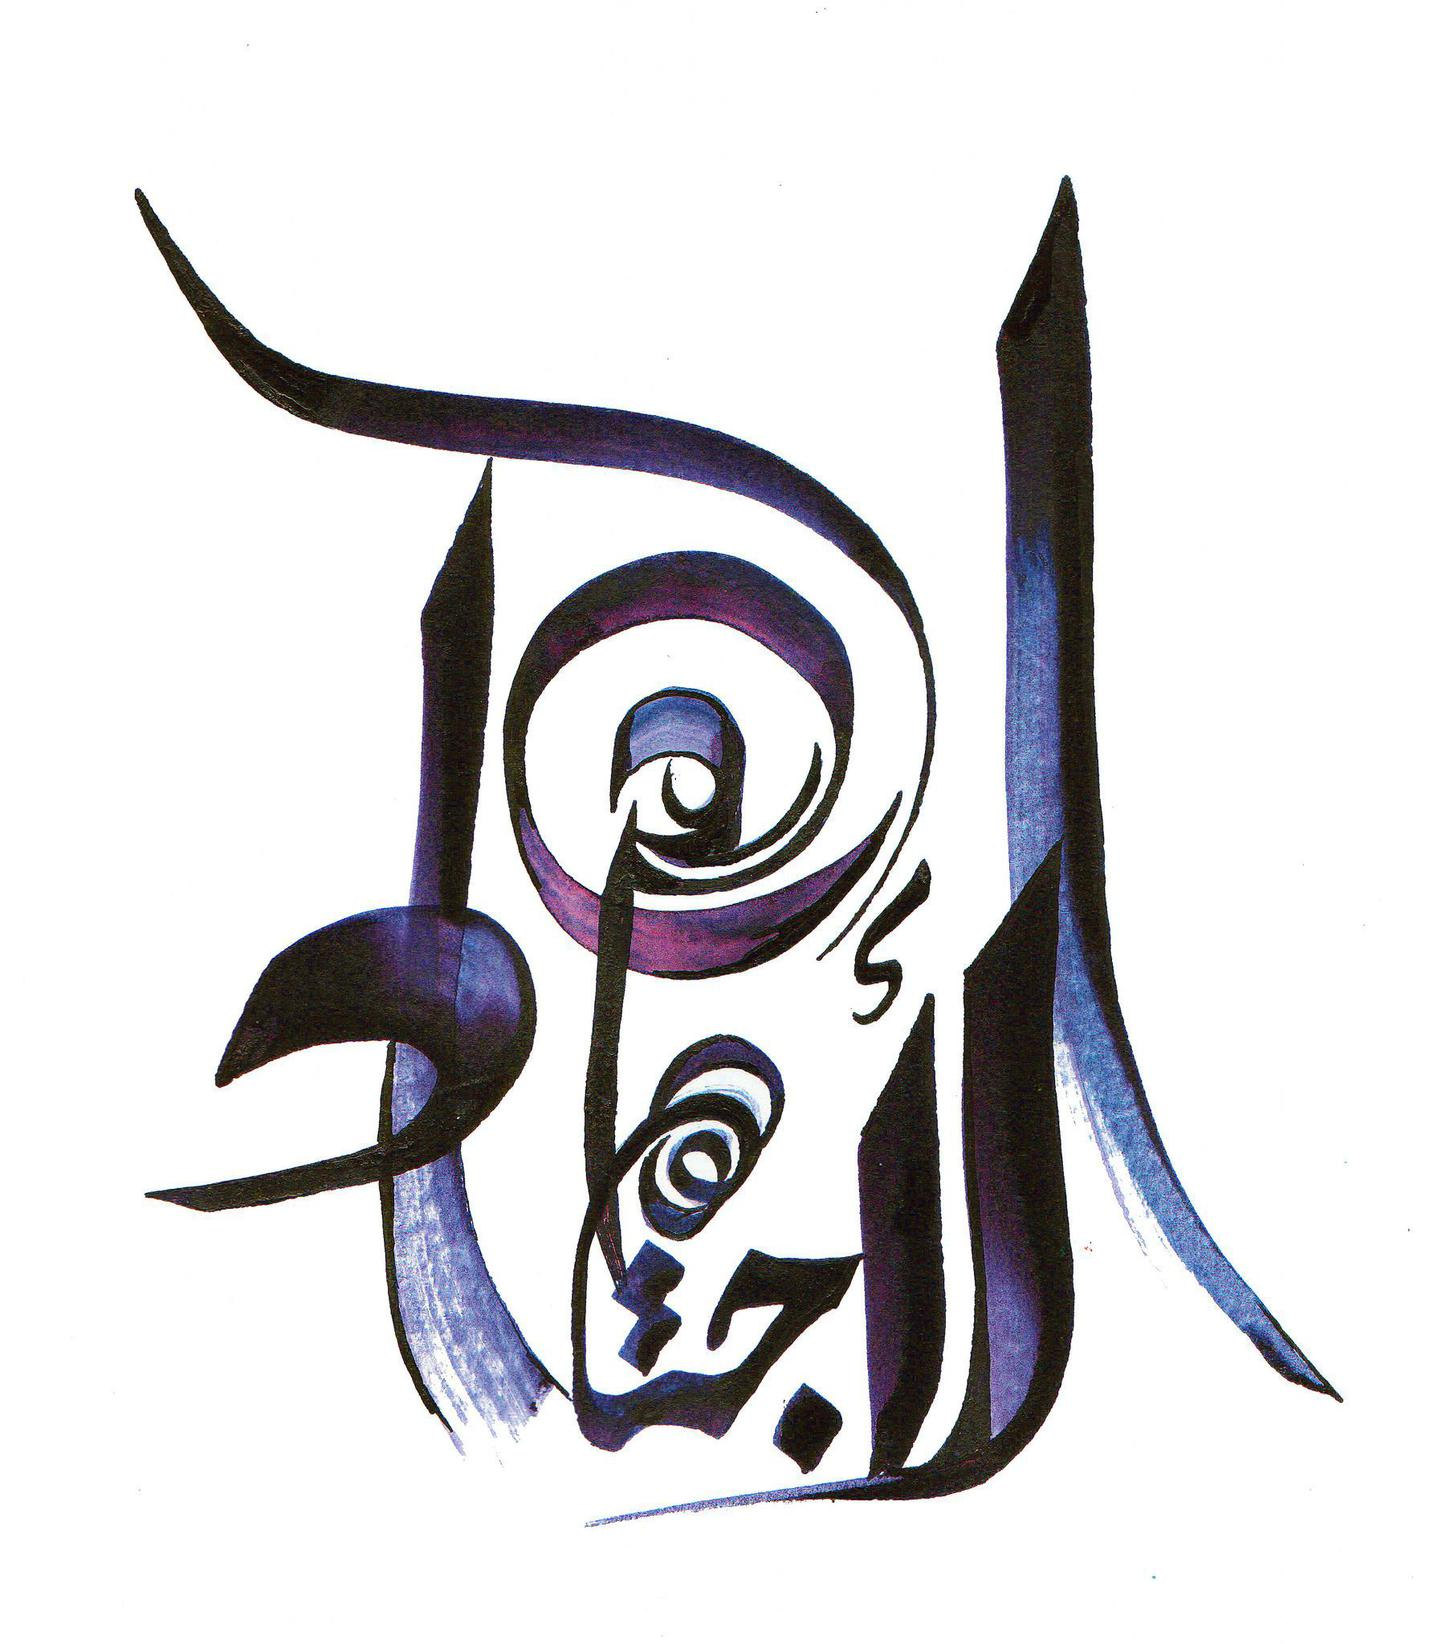
\includegraphics[width=\textwidth]{Images/image009.png}
\begin{Def}[iǧtihād]
L'ijtihad désigne l'étude raisonnée des textes sacrés et leur
interprétation.
\end{Def}
\begin{cite}
«On prétend aujourd'hui qu'au
X\textsuperscript{e}~siècle, la~\emph{« porte de l'interprétation »}~se
serait fermée, mais ce moment n'a jamais existé. Ce qui s'est passé est
très différent. Les premiers convertis à l'islam étaient des membres de
l'élite, des penseurs et des théologiens. À partir de la fin du
IX\textsuperscript{e}~siècle, ils ont été concurrencés par des convertis
de condition plus ordinaire. C'est ce qu'on pourrait appeler l'islam des
boutiquiers. Ces nouveaux croyants n'avaient pas besoin de grandes
réflexions philosophiques, mais de juridisme et de règles de
vie. L'ijtihad, pratiqué par les intellectuels, va s'effacer au profit
d'un islam plus juridique. À partir du moment où le sunnisme prend le
dessus, l'ijtihad va être endigué. Mais l'idée qu'il y aurait eu une
décision de clore l'interprétation des textes est fausse. Aucune société
ne peut fermer quoi que ce soit sur le plan idéologique. » Jacqueline Chabbi
\end{cite}


\begin{cite}
« Ce mot a plusieurs sens. Quand un enfant marche bien à l'école, qu'il
est travailleur et qu'il réussit, on dit qu'il est~\emph{``ijtihad''}.
Mais  \emph{ijtihad}~désigne aussi le moment où l'on dit que
l'interprétation des textes s'est arrêtée, au Moyen Âge. J'ai dessiné un
espace fermé par deux lignes mais qui reste ouvert en haut. Au centre,
j'ai placé comme un tourbillon. Si on veut s'en sortir, c'est par le
haut. Si on suit la spirale, il y a même une possibilité de s'envoler,
mais c'est toujours par le haut\ldots{} » Hassan Massoudy
\end{cite}



\vide{i.-chronologie-de-la-ruxe9vuxe9lation}{%
\section{Chronologie de la révélation
}\label{i.-chronologie-de-la-ruxe9vuxe9lation}}

La révélation coranique a duré vingt-deux années. Or, cette révélation
n'est pas sans lien avec les contextes dans lesquels se trouve Muḥammad.
Il existe donc une histoire de la révélation. On distingue classiquement
deux grandes périodes~: celle de La Mecque qui va du premier jour de la
révélation jusqu'à l'hégire (\emph{hiǧra}), c'est-à-dire l'exil,
l'émigration de Muḥammad vers l'oasis de Yathrib, Médine. Cette première
période va durer 13 années. La seconde période est donc celle de Médine
avec la révélation des versets dits «~médinois~».

L'\emph{hiǧra} \TArabe{(هجرة)}  atteste des difficultés rencontrées par Muḥammad à
La Mecque, mais aussi de la naissance et de l'organisation de la
communauté dans un contexte multi-religieux~: à Médine, Muḥammad
rencontre des juifs, des chrétiens, des polythéistes.

Cette première communauté musulmane est constituée

* des \emph{muhāǧirūn (émigrés)}, c'est-à-dire de ceux qui viennent de
La Mecque, qui ont effectué l'Hégire.

*~des \emph{anṣār}, c'est-à-dire des compagnons de Yathrib qui vont
suivre le Prophète. La distinction entre \emph{anṣār} et
\emph{muhāǧirūn} va avoir des incidences politiques au moment de la mort
du Prophète. «~Son corps n'était pas encore lavé~» selon la Chronique de
Ṭabarī\sn{Ṭabarī, \emph{La Chronique}, \emph{Volume II, Mohammed
  le sceau des prophètes}, Paris, Actes-Sud, p. 349.} (839-923) que déjà
éclatait une dispute entre \emph{anṣār} et \emph{muhāǧirūn}, ces
derniers affirmant que le calife devait venir de la tribu des Qurayš (à
laquelle appartenait Muḥammad). Certains lexicographes font remarquer
qu'\emph{anṣār} vient de la racine NSR, nazaréens. Ils notent que dans
le Coran, le terme apparaît pour la première fois en lien avec les
apôtres de Jésus~: S. 61, 14 «~Ô vous qui avez cru! Soyez les alliés
d'Allah, à l'instar de ce que Jésus fils de Marie a dit aux apôtres:
`Qui sont mes alliés pour la cause d'Allah?' - Les apôtres dirent~:
`Nous sommes les alliés d'Allah'. Un groupe des Enfants d'Israël crut,
tandis qu'un groupe nia~; nous aidâmes donc ceux qui crurent contre leur
ennemi, et ils triomphèrent~».

* des \emph{munāfiqūn}, c'est-à-dire ceux qui à Médine prétendent
rejoindre l'\emph{umma} mais qui y restent, dans le fond, extérieurs. Ce
sont les hypocrites.

Dans ce contexte, les savants musulmans vont établir des listes afin de
dresser la chronologie de chaque verset. Savoir distinguer ce qui relève
des versets mecquois ou des versets médinois a des incidences sur la
question de l'abrogation, en sachant que selon les sciences coraniques,
ce qui est postérieur abroge ce qui est antérieur.
\begin{Def}[Verset abrogeant abrogé]
\label{mansûkh}
Les expressions arabes mansûkh (arabe :\TArabe{
مَنْسوخ 
}
[mansūḫ], abrogé) et nâsikh( \TArabe{
ناسِخ 
}
[nāsiḫ], abrogeant, abrogatif, abrogatoire), correspondent en français aux notions de verset abrogé et de verset abrogatif du Coran. Certains versets du Coran sont dits mansûkh lorsqu'on considère qu'une révélation ultérieure dans un autre verset vient le modifier ou le corriger. Ce verset correctif est alors dit nâsikh, verset abrogatif.
\end{Def}
Pour procéder à
l'abrogation, il faut donc savoir si le verset est mecquois ou médinois.
Autre incidence~: les causes de la révélation. C'est en connaissant les
causes de la révélation d'un verset qu'on peut en effet caractériser
s'il est de La Mecque ou de Médine.

\vide{les-versets-de-la-mecque-et-les-versets-de-muxe9dine}{%
\subsection{Les versets de La Mecque et les versets de
Médine}\label{les-versets-de-la-mecque-et-les-versets-de-muxe9dine}}

\vide{section-20}{%
{{\includegraphics[width=1.34722in,height=1.01046in]{Images/image51.jpeg}}{}}\label{section-20}}

Disons d'emblée que la révélation coranique a commencé près de La
Mecque, dans la grotte de Ḥirā'. Le Coran lui a continué à lui être
révélé jusqu'à sa mort. Pour connaître si un verset est mecquois ou
médinois, on va s'appuyer sur les compagnons~: \emph{un tel a entendu
que Muḥammad, alors qu'il été à La Mecque, a récité le verset\ldots{}
etc.}

Pour autant, il n'y a pas toujours consensus parmi les compagnons, et
par suite, parmi les savants, pour savoir ce qui relève de La Mecque ou
de Médine. Ces divergences ne portent pas tant sur les sourates que sur
des versets de ces sourates. Une sourate en effet, peut contenir des
versets mecquois et des versets médinois.

\vide{lislam-comme-systuxe8me-religieux-est-achevuxe9.-liux1e7tihux101d-na-pas-uxe9tuxe9-aboli-et-il-est-restuxe9-intuxe9gruxe9-uxe0-la-ruxe9flexion-savante.-en-revanche-le-taqlux12bd-que-les-ruxe9formateurs-ont-remis-en-cause.}{%
\subsubsection{l'islam, comme système religieux, est achevé.
l'iǧtihād~n'a pas été aboli et il est resté intégré à la réflexion
savante. En revanche, le taqlīd~que les~réformateurs ont remis en
cause.}\label{lislam-comme-systuxe8me-religieux-est-achevuxe9.-liux1e7tihux101d-na-pas-uxe9tuxe9-aboli-et-il-est-restuxe9-intuxe9gruxe9-uxe0-la-ruxe9flexion-savante.-en-revanche-le-taqlux12bd-que-les-ruxe9formateurs-ont-remis-en-cause.}}

On trouve dans la plupart des ouvrages de \emph{`ulūm al-qur'ān} (le mot
est traduit dans le titre, je dis ça au cas où\ldots) une liste des
sourates mecquoises et médinoises\sn{Par exemple, Zarkašī,
  \emph{al-Burhān fī `ulūm al-Qur'ān}, Cairo, 1958, Vol.1, p. 193.}. Ces
listes sont aussi accompagnées d'un ordre chronologique des sourates.
Mais il faut savoir que cet ordre est sujet à discussion puisque selon
les auteurs, il peut différer. Cela n'est pas sans conséquence\ldots{}

Pour déterminer l'origine d'un verset, il faut donc procéder à
l'\emph{iǧtihād}. Dans cet esprit, on va distinguer des caractéristiques
spécifiques à chaque époque~: thématique, expressions, etc.

\vide{caractuxe9ristiques-des-versets-mecquois}{%
\subsubsection{{Caractéristiques des versets
mecquois
}}\label{caractuxe9ristiques-des-versets-mecquois}}

\vide{appel-uxe0-la-conversion}{%
\paragraph{Appel à la conversion}\label{appel-uxe0-la-conversion}}

La prédication mecquoise se caractérise par un appel à la conversion. Il
y a quelque chose de Jean-Baptiste qui appelle à se convertir. Il s'agit
d'abandonner les idoles, les faux dieux et de se tourner vers le Dieu
unique Allāh.

\vide{dimension-eschatologique}{%
\paragraph{Dimension eschatologique}\label{dimension-eschatologique}}

Ces versets ont aussi une dimension eschatologique~qui tend à rendre
plus urgente la conversion~: la fin des temps est proche.

\vide{vie-droite}{%
\paragraph{Vie droite}\label{vie-droite}}

Il s'ensuit un appel à mener une vie droite et juste conformément au
chemin tracé par Dieu (Allāh).

\vide{les-thuxe9matiques-des-versets-muxe9dinois}{%
\subsubsection{{  les thématiques des versets
médinois
} }\label{les-thuxe9matiques-des-versets-muxe9dinois}}

 
\paragraph{Abraham}\label{abraham}

le thème d'Abraham comme «~Père des croyants~» où Abraham est dit
d'une part \emph{ḥanīf}, c'est-à-dire monothéiste exclusif, mais aussi
\emph{muslim}, c'est-à-dire soumis, abandonné à Dieu, et ni juif ni
chrétien, date de la période médinoise.

\begin{longtable}{p{5cm}p{5cm}}
\toprule
\endhead
«~Abraham n'était ni juif ni chrétien, mais il était un monothéiste
exclusif, abandonné à Dieu~; il n'était pas au nombre des polythéistes.
Les hommes les plus proches d'Abraham sont vraiment ceux qui l'ont
suivi, ainsi que ce Prophète et ceux qui ont cru~». (S. 3, 67-68). &
\TArabe{مَا كَانَ إِبْرَاهِيمُ يَهُودِيًّا وَلَا نَصْرَانِيًّا وَلَكِنْ
كَانَ حَنِيفًا مُسْلِمًا وَمَا كَانَ مِنَ الْمُشْرِكِينَ إِنَّ أَوْلَى
النَّاسِ بِإِبْرَاهِيمَ لَلَّذِينَ اتَّبَعُوهُ وَهَذَا النَّبِيُّ
وَالَّذِينَ آَمَنُوا وَاللَّهُ وَلِيُّ الْمُؤْمِنِينَ} \\
\bottomrule
\end{longtable}

Ce verset a bien sûr donné lieu à de multiples commentaires. Il est
souvent interprété dans le sens où Abraham est dépositaire de la
religion originelle avant son altération par les juifs et les chrétiens.
Souvent ne veut pas pour autant dire toujours. Il y a d'autres
lectures\ldots{}

Sur la \emph{ḥanīfiyya}, c'est-à-dire cette affirmation d'une foi
exclusive, sans associationnisme (\emph{širk}), le Coran raconte un
dialogue entre Dieu et Abraham\emph{~}:

\begin{quote}
    «~Ainsi avons-Nous montré à Abraham le royaume des cieux et de la terre
afin qu'il soit de ceux qui croient avec conviction. Lorsque la nuit
l'enveloppa, il vit une étoile et dit : « Voilà mon Seigneur ! » Puis,
lorsqu'elle disparut, il dit : « Je n'aime pas les choses qui
disparaissent~». Il vit ensuite la lune se lever et dit : « Voilà mon
Seigneur ! » Puis, lorsqu'elle disparut, il dit : « Si mon Seigneur ne
me guide pas, je serai assurément du nombre des égarés. » Voyant enfin
le soleil levant, il dit : « Voilà mon Seigneur ! Celui-ci est plus
grand~». Puis, lorsqu'il disparut, il dit : « Ô mon peuple, je désavoue
tout ce que vous associez à Dieu. Je tourne mon visage comme un vrai
croyant vers Celui qui a créé les cieux et la terre, et je ne suis pas
de ceux qui Lui donnent des associés » (S. 6, 76-79) & \TArabe{فَلَمَّا
جَنَّ عَلَيْهِ اللَّيْلُ رَأَى كَوْكَبًا قَالَ هَذَا رَبِّي فَلَمَّا
أَفَلَ قَالَ لَا أُحِبُّ الْآَفِلِينَ (}76\TArabe{) فَلَمَّا رَأَى الْقَمَرَ
بَازِغًا قَالَ هَذَا رَبِّي فَلَمَّا أَفَلَ قَالَ لَئِنْ لَمْ يَهْدِنِي
رَبِّي لَأَكُونَنَّ مِنَ الْقَوْمِ الضَّالِّينَ (}77\TArabe{) فَلَمَّا رَأَى
الشَّمْسَ بَازِغَةً قَالَ هَذَا رَبِّي هَذَا أَكْبَرُ فَلَمَّا أَفَلَتْ
قَالَ يَا قَوْمِ إِنِّي بَرِيءٌ مِمَّا تُشْرِكُونَ (}78\TArabe{) إِنِّي
وَجَّهْتُ وَجْهِيَ لِلَّذِي فَطَرَ السَّمَاوَاتِ وَالْأَرْضَ حَنِيفًا
وَمَا أَنَا مِنَ الْمُشْرِكِينَ (}79\TArabe{) وَحَاجَّهُ قَوْمُهُ قَالَ
أَتُحَاجُّونِّي فِي اللَّهِ وَقَدْ هَدَانِ وَلَا أَخَافُ مَا تُشْرِكُونَ
بِهِ إِلَّا أَنْ يَشَاءَ رَبِّي شَيْئًا وَسِعَ رَبِّي كُلَّ شَيْءٍ
عِلْمًا أَفَلَا ت

َتَذَكَّرُونَ} \\

\end{quote}
Ce dialogue est connu dans le monde biblique. Il se retrouve dans des
écrits juifs, chrétiens et judéo-chrétiens~: Ainsi par exemple, dans
\emph{L'Apocalypse d'Abraham}\sn{~\emph{L'Apocalypse d'Abraham}
  est un livre apocryphe dont on dispose de manuscrits en roumain et en
  slave. L'original devait être une traduction grecque de l'hébreu ou de
  l'araméen. Le texte est daté du premier siècle, sans doute après la
  destruction du Temple de Jérusalem par les Romains en 70. Apocalypse
  d'Abraham car il est question de la vie du patriarche et de son
  dialogue avec Dieu mais aussi d'une ascension et de visions où les
  anges* jouent un rôle important, notamment celle du char céleste de
  Dieu (cf. Ez 1).} : «~Plus que la terre, j'appellerai digne de
vénération le soleil car il éclaire de ses rayons le monde et les
différentes atmosphères. Mais celui-là non plus je ne le placerai pas
parmi les dieux, car la nuit, sa course est assombrie par les nuées~»
(7, 1, 7).

Le terme \emph{ḥanīf} est employé par deux fois pour Muḥammad (S. 10,
105 et 30, 30), Muḥammad étant lui-même chargé de détruire les idoles de
la Ka`ba.

L'injonction est aussi adressée aux Gens du Livre à qui il fut demandé
seulement d'agir «~comme des \emph{ḥunafā'} (\emph{ḥunafā' est le
pluriel de ḥanīf}) et non comme des polythéistes~» (S. 22, 31).

\vide{falsification-des-uxe9critures}{%
\paragraph{Falsification des
écritures}\label{falsification-des-uxe9critures}}

- toute la théologie coranique relative à la falsification des
écritures~:
\begin{quote}
    


«~Comment pouvez-vous désirer qu'ils croient avec vous, alors que
certains d'entre eux ont falsifié sciemment~la Parole de Dieu, après
l'avoir entendue~?» (S. 2, 75) est de Médine. & \TArabe{أَفَتَطْمَعُونَ أَنْ
يُؤْمِنُوا لَكُمْ وَقَدْ كَانَ فَرِيقٌ مِنْهُمْ يَسْمَعُونَ كَلَامَ
اللَّهِ ثُمَّ يُحَرِّفُونَهُ مِنْ بَعْدِ مَا عَقَلُوهُ وَهُمْ
يَعْلَمُون} \\
\end{quote}

\vide{vie-uxe0-muxe9dine}{%
\paragraph{Vie à Médine}\label{vie-uxe0-muxe9dine}}

- De même, les prescriptions relatives à la manière de vivre datent de
Médine~:

\begin{longtable}{p{5cm}p{5cm}}
\toprule
\endhead
«~Il n'appartient pas à un croyant ou une croyante, une fois qu'Allah ou
Son messager ont décidé une chose d'avoir encore le choix dans leur
façon d'agir. Et quiconque désobéit à Allah et son messager s'est égaré
certes, d'un égarement évident~» (S. 33, 36). & \TArabe{وَمَا كَانَ
لِمُؤْمِنٍ وَلَا مُؤْمِنَةٍ إِذَا قَضَى اللَّهُ وَرَسُولُهُ أَمْرًا أَنْ
يَكُونَ لَهُمُ الْخِيَرَةُ مِنْ أَمْرِهِمْ وَمَنْ يَعْصِ اللَّهَ
وَرَسُولَهُ فَقَدْ ضَلَّ ضَلَالًا مُبِينًا} \\
\bottomrule
\end{longtable}

Toutes les questions relatives au statut social et légal sur le mariage,
le divorce, les héritages, les punitions\ldots{} sont aussi de Médine.

Outre les différences thématiques, on trouve différentes
expressions~propres à chaque période. Ainsi, les adresses \textbf{«~Ô
vous qui croyez~» ou «~Ô gens du Livre~» caractérisent les sourates
médinoises} tandis que \textbf{«~Ô vous les gens~» est plutôt
mecquoise}.

\vide{importance-de-la-chronologie}{%
\subsection{Importance de la
chronologie}\label{importance-de-la-chronologie}}

Dans la mesure où le Coran ne suit pas l'ordre chronologique, en quoi
est-il si important du point de vue des sciences coraniques de connaître
cette chronologie et la nature de la sourate (mecquoise ou médinoise)~?

Il s'avère que cette connaissance a des conséquences décisives dans la
référence des versets selon les situations posées. On se souviendra que
les versets mecquois «~parlent~» tout particulièrement aux musulmans
vivant dans une situation difficile et d'hostilité à leur égard. Au
contraire, dans le cadre d'une société musulmane, on s'appuiera
spécifiquement sur les versets de Médine.

Par ailleurs, la chronologie permet de mieux saisir l'évolution des
positions du Coran sur une même question, l'évolution des pratiques, à
l'instar par exemple de la consommation d'alcool.

Enfin, la chronologie permet de distinguer \textbf{les versets
abrogeants des versets abrogés}, c'est-à-dire en cas de contradiction,
celui qui abroge l'autre. Le critère retenu, comme nous le verrons, est
chronologique~: le dernier verset révélé abroge celui qui le précède.


\section{La question de l'abrogation
}\label{ii.-la-question-de-labrogation}

La question de l'abrogation est essentielle dans l'exégèse coranique.
Tandis que le Coran est compris comme une guidance universelle, la
chronologie du Coran montre l'existence d'une progressivité de la
révélation. Sur ce point, il existe selon les commentateurs une
pédagogie divine.

Pour autant, sa pratique n'est pas sans difficulté. Elle est au cœur des
débats contemporains sur l'exégèse coranique dans la mesure où
l'abrogation s'effectue dans le sens chronologique de la révélation. Or,
il s'ensuit que les versets médinois, c'est-à-dire les plus prescriptifs
et légalistes, abrogent les versets plus universels de La Mecque.
Au-delà même de la question versets médinois / versets mecquois, le
verset «~Pas de contrainte en religion~» (S.2, 256) qui est un verset
médinois, est-il abrogé par les versets dits \emph{de l'épée} (S,9,5),
eux aussi médinois~qui lui sont postérieurs ? C'est ce que soutient par
exemple le savant saoudien Ibn Bāz (1910-1999).

\begin{longtable}{p{5cm}p{5cm}}
\toprule
Nulle contrainte en religion! Car le bon chemin s'est distingué de
l'égarement. Donc, quiconque mécroit au Rebelle tandis qu'il croit en
Allah saisit l'anse la plus solide, qui ne peut se briser. Et Allah est
Audient et Omniscient. (S.2, 256) & \TArabe{لَا إِكْرَاهَ فِي الدِّينِ قَد
تَّبَيَّنَ الرُّشْدُ مِنَ الْغَيِّ فَمَن يَكْفُرْ بِالطَّاغُوتِ
وَيُؤْمِن بِاللَّهِ فَقَدِ اسْتَمْسَكَ بِالْعُرْوَةِ الْوُثْقَى لَا
انفِصَامَ لَهَا وَاللَّهُ سَمِيعٌ عَلِيمٌ} \\
\midrule
\endhead
Après que les mois sacrés expirent, tuez les associateurs où que vous
les trouviez (S,9,5),. Capturez-les, assiégez-les et guettez-les dans
toute embuscade. Si ensuite ils se repentent, accomplissent la Salât et
acquittent la Zakât, alors laissez-leur la voie libre, car Allah est
Pardonneur et Miséricordieux. &\TArabe{ فَإِذَا انسَلَخَ الْأَشْهُرُ الْحُرُمُ
فَاقْتُلُوا الْمُشْرِكِينَ حَيْثُ وَجَدتُّمُوهُمْ وَخُذُوهُمْ
وَاحْصُرُوهُمْ وَاقْعُدُوا لَهُمْ كُلَّ مَرْصَدٍ فَإِن تَابُوا
وَأَقَامُوا الصَّلَاةَ وَآتَوُا الزَّكَاةَ فَخَلُّوا سَبِيلَهُمْ إِنَّ
اللَّهَ غَفُورٌ رَّحِيمٌ 
} \\
\bottomrule
\end{longtable}

\vide{un-principe-juridique-fonduxe9-sur-le-coran}{%
\subsection{{ Un principe juridique fondé sur le
Coran~?
}}\label{un-principe-juridique-fonduxe9-sur-le-coran}}

On distingue donc entre verset abrogé (\emph{ayāh mansūḫa}) et verset
abrogeant (\emph{ayāh nāsiḫa}). Ce principe repose sur le verset
coranique suivant~:

\begin{longtable}{p{5cm}p{5cm}}
\toprule
\endhead
«~nous n'abrogeons aucun verset. Nous n'en faisons oublier aucun sans le
remplacer par un autre qui soit meilleur ou équivalent~» (S. 2, 106). &
\TArabe{مَا نَنْسَخْ مِنْ آَيَةٍ أَوْ نُنْسِهَا نَأْتِ بِخَيْرٍ مِنْهَا أَوْ
مِثْلِهَا} \\
\bottomrule
\end{longtable}

Cependant, l'analyse littéraire a montré que le contexte de ce verset ne
renvoie pas au Coran mais aux Écritures antérieures\sn{Michel
  \textsc{Cuypers}, «~Le verset de l'abrogation (2, 106) dans son
  contexte rhétorique~» dans Mehdi Azaiez (dir.) avec la collaboration
  de Sabrina \textsc{Mervin}, \emph{Le Coran : nouvelles approches},
  Paris, CNRS, 2013.}. \textbf{Dieu n'abroge pas les versets de la Torah
sans les remplacer par d'autres~: les versets coraniques}. Autrement
dit, on ne trouverait pas dans le Coran une justification de
l'abrogation du Coran par le Coran. Certains théologiens l'ont aussi
noté, à l'exemple du fondamentaliste Mawdudi (1903-1979)\sn{\textsc{Mawdudi},
  \emph{Comprendre le Coran}.}. On a le même problème avec la théologie
protestante et le principe fondamental de la \emph{sola scriptura}. Mais
où l'Écriture dit-elle que pour une question théologique, on ne peut
recourir pour répondre qu'à l'Écriture~?

Cette question n'est pas anecdotique et peut avoir de grandes
répercussions dans la refondation de la pensée musulmane à laquelle
appellent bien des penseurs musulmans.

\vide{un-enjeu-thuxe9ologique-dieu-peut-il-se-contredire}{%
\subsection{{Un enjeu théologique~: Dieu peut-il se
contredire~?
}}\label{un-enjeu-thuxe9ologique-dieu-peut-il-se-contredire}}

Le fait que des versets coraniques ne tiennent pas la même position
ouvre à une difficulté majeure : Comment la Parole de Dieu, immuable,
éternelle, peut-elle contenir des versets contradictoires~? Dieu ne
pouvant être versatile, comment sa Parole pourrait-elle l'être ? N'y
a-t-il pas le risque d'affaiblir et de remettre en cause l'affirmation
de la nature parfaite du Coran~?

Pour les mu`tazilites, c'est-à-dire les rationalistes, le problème ne se
pose pas~car la Loi donnée par Dieu suit l'intérêt (\emph{al-maṣlaha}).
Chaque contexte est singulier et Dieu donne un commandement qui guide la
communauté dans le sens qui lui est le plus profitable. Ce principe
exégétique a influencé la jurisprudence islamique~: au
11\textsuperscript{ème} siècle, le légiste al-Māwardī (974-1058) écrit~:

«~L'intérêt diffère selon les époques~: un statut shariatique peut très
bien avoir été dans le sens de son intérêt à une époque et un autre,
abrogeant le précédent, aller dans son sens à une autre époque. Chacun
des deux statuts présente un intérêt en son temps, même s'ils sont
antinomiques~»\sn{~Eric \textsc{Chaumont}, «~Abrogation~», dans
  Amir \textsc{Moezzi}, \emph{Dictionnaire du Coran}, \emph{op. cit}.,
  p. 14.}.

Une conséquence est d'introduire dans la Loi divine une distance
critique et un principe de relativisme. La communauté n'applique donc
pas une Loi dans sa littéralité, mais doit d'abord se poser la question
de l'intérêt pour elle-même, dans un contexte géographique et politique
propre. Vous voyez que bien sûr, les fondamentalistes y voient un risque
d'instrumentaliser la Loi divine et de lui ôter son caractère sacré. Ils
accusent les rationalistes et avec eux les nouveaux penseurs de ne
prendre dans la Loi que ce qui les arrange\ldots{} D'autres, plus
contempteurs, diront avec méfiance qu'une lecture souple de la loi ne
peut être que temporaire et s'inscrire dans une stratégie progressive
d'islamisation\ldots{} C'est compliqué, mais il faut connaître toutes
ces discussions et subtilités en arrière-fond de la question de
l'abrogation. Nous y reviendrons quand nous aborderons le droit
islamique (\emph{fiqh}).


\mn{{ L'acharisme~est une
école~{théologique}~de
l'{islam}, fondée
par~{Abu
Al-Hasan
al-ʾAshʿarī}~({873}-{935}).
(\TArabe{الأشعرية}~). Cette école de pensée se répandit très vite et devint
l'école théologique majoritaire. D'abord adepte du~mu'tazilisme~il~s'en
sépara au moins sur deux points
essentiels~:} 
\begin{itemize}
    \item il affirme que l'homme est libre de ses actions mais
c'est Dieu qui crée ses actes (bons ou
mauvais)
\item Il déclare que le~Coran~est incréé car, étant la Parole de Dieu lui-même, elle fait donc partie de lui
\end{itemize}}


Pour le courant théologique \textbf{asharite}, une telle thèse est
impossible : \textbf{Dieu ne peut être versatile dans sa volonté}.
\textbf{Al-Rāzī} (m. 1209), le grand commentateur du Coran, répond en
soulignant la \textbf{dimension pédagogique de Dieu}~: Dieu ne se
contredit pas mais prend l'homme tel qu'il est et le fait avancer à son
rythme.
\mn{Al-razi, théologien musulman de rite chaféite, est né à
Ray ou 1150, et mort en 1210 à Hérat. Musulman d'obédience sunnite, il
écrit le Le Grand Commentaire du Coran (aussi connu sous le titre Les
Clés de l'invisible). fervent défenseur de la doctrine de
l'unicité}

\vide{abrogation-et-falsification}{%
\subsection{Abrogation et
falsification}\label{abrogation-et-falsification}}

L'abrogation concerne aussi et surtout les écritures antérieures. Pour
les musulmans, les livres donnés aux Juifs et chrétiens ont été altérés,
falsifiés (\emph{taḥrīf}, S. 5, 13) et Dieu leur a substitué l'Écriture
authentique. C'est le \emph{tabdīl} (S. 7, 162) qui consiste donc à
\textbf{remplacer l'erreur par la vérité.}

La dénonciation de la falsification des Écritures prend trois formes. Le
Coran accuse les gens du Livre de ne pas tout dire, d'avoir fabriqué de
faux versets, ou encore d'en avoir effacé certains.

\begin{itemize}
\item
  Ne pas tout dire~: «~Ô Détenteurs de l'Écriture~! Pourquoi
  travestissez-vous la Vérité au moyen du faux~? Pourquoi tenez-vous
  secrète la Vérité, alors que vous savez~? (3, 71).
\end{itemize}

\TArabe{يَا أَهْلَ الْكِتَابِ لِمَ تَلْبِسُونَ الْحَقَّ بِالْبَاطِلِ
وَتَكْتُمُونَ الْحَقَّ وَأَنْتُمْ تَعْلَمُونَ}

\begin{itemize}
\item
  Avoir fabriqué un faux~: «~malheur à ceux qui de leurs propres mains
  composent un livre, puis le présentent comme venant d'Allah pour en
  tirer un vil profit~! Malheur à eux à cause de ce qu'ils en
  profitent~» (S. 2, 79). On retrouve ici le cœur de la polémique
  anti-chrétienne où l'Évangile aurait été dénaturé.
\end{itemize}

\TArabe{فَوَيْلٌ لِلَّذِينَ يَكْتُبُونَ الْكِتَابَ بِأَيْدِيهِمْ ثُمَّ
يَقُولُونَ هَذَا مِنْ عِنْدِ اللَّهِ لِيَشْتَرُوا بِهِ ثَمَنًا قَلِيلًا
فَوَيْلٌ لَهُمْ مِمَّا كَتَبَتْ أَيْدِيهِمْ وَوَيْلٌ لَهُمْ مِمَّا
يَكْسِبُونَ}

\begin{itemize}
\item
  Avoir effacé~: «~Ô détenteurs de l'Écriture~! notre messager est venu
  à vous, vous exposant une grande partie de l'Écriture que vous cachiez
  et aviez effacée aussi une grande partie de celle-ci~» (S. 5, 15).
\end{itemize}

\TArabe{يَا أَهْلَ الْكِتَابِ قَدْ جَاءَكُمْ رَسُولُنَا يُبَيِّنُ لَكُمْ
كَثِيرًا مِمَّا كُنْتُمْ تُخْفُونَ مِنَ الْكِتَابِ وَيَعْفُو عَنْ
كَثِيرٍ قَدْ جَاءَكُمْ مِنَ اللَّهِ نُورٌ وَكِتَابٌ مُبِينٌ}

L'argument théologique de la falsification des écritures n'est pas
nouveau. Il a déjà été utilisé par des chrétiens à l'encontre des juifs.
Mani, le philosophe prophète du deuxième siècle, y a eu aussi recours.

\vide{quels-sont-les-versets-abrogeants-et-abroguxe9s}{%
\subsection{{Quels sont les versets abrogeants~et
abrogés ?
}{ Quels sont les versets abrogeants~et abrogés ? }}\label{quels-sont-les-versets-abrogeants-et-abroguxe9s}}

Là encore, les spécialistes en \emph{`ulūm al-qur'ān}  dressent la
liste des versets abrogés ou abrogeants. Elles ne sont pas identiques.

\mn{{Abū l-Fadl al-Suyūtī, né
en~{1445}~au Caire, est un
savant égyptien connu pour son œuvre abondante. Il fut un éminent
savant~Shâfi'ite, un théologien~Ash'arite~de renom. il serait né dans la
bibliothèque familiale ce qui lui valut son surnom de «~fils des
livres~» (ibn al-kutub). D'une mémoire prodigieuse, il connaissait par
cœur quelque deux cent mille hadiths. Il se rattacha à la~ṭarīqa
shādhiliyya~et prôna l'équilibre entre la Loi et la Voie. On lui
reprocha notamment son emploi de l'ijtihād~mais sans qu'il fut jugé
condamnable. D'une façon générale, il rejeta le pouvoir des Mamelouks.
Il prôna la complémentarité de l'exotérisme et
du~ {soufisme}. On lui
attribue jusqu'à 981
ouvrages.}}

Al-Suyūtī (1445-1505) dans son \emph{Itqān} (cet ouvrage est étudié par
tous les musulmans qui font des sciences islamiques pour devenir imam)
note qu'il existe 21 passages coraniques qui ont été abrogés et il
précise que tous ceux qui en désignent d'autres sont dans l'erreur. Cet
ouvrage n'est pas encore traduit en français, mais le Père Michel
Lagarde, père blanc qui a enseigné au PISAI, en prépare la traduction.
Elle vient de paraître en novembre 2017, mais je ne l'ai pas encore pu
consulter. Je vous signale que pour al-Suyūtī, le verset «~Pas de
contrainte en religion~» (S.2, 256) n'est pas abrogé.

On trouve aussi des listes plus restreintes. Shah Waliullah (fameux
musulman indien mort en 1759) ne retient à partir de la liste de
al-Suyūtī que 5 versets~:

\begin{quote}
Abrogé 2, 180, abrogeant~: 4, 11, 12
\end{quote}

\begin{longtable}{p{4cm}p{8cm}}

\toprule
Abrogé 2, 180 & abrogeant~ 4, 11, 12\\
\midrule
\endhead
On vous a prescrit, quand la mort est proche de l'un de vous et s'il
laisse des biens, de faire un testament en règle en faveur de ses père
et mère et de ses plus proches. C'est un devoir pour les pieux. & Voici
ce qu'Allah vous enjoint au sujet de vos enfants: au fils, une part
équivalente à celle de deux filles. S'il n'y a que des filles, même plus
de deux, à elles alors deux tiers de ce que le défunt laisse. Et s'il
n'y en a qu'une, à elle alors la moitié. Quant aux père et mère du
défunt, à chacun d'eux le sixième de ce qu'il laisse, s'il a un enfant.
S'il n'a pas d'enfant et que ses père et mère héritent de lui, à sa mère
alors le tiers. Mais s'il a des frères, à la mère alors le sixième,
après exécution du testament qu'il aurait fait ou paiement d'une dette.
De vos ascendants ou descendants, vous ne savez pas qui est plus près de
vous en utilité. Ceci est un ordre obligatoire de la part d'Allah, car
Allah est, certes, Omniscient et Sage.

Et à vous la moitié de ce que laissent vos épouses, si elles n'ont pas
d'enfants. Si elles ont un enfant, alors à vous le quart de ce qu'elles
laissent, après exécution du testament qu'elles auraient fait ou
paiement d'une dette. Et à elles un quart de ce que vous laissez, si
vous n'avez pas d'enfant. Mais si vous avez un enfant, à elles alors le
huitième de ce que vous laissez après exécution du testament que vous
auriez fait ou paiement d'une dette. Et si un homme, ou une femme meurt
sans héritier direct, cependant qu'il laisse un frère ou une sœur, à
chacun de ceux-ci alors, un sixième. S'ils sont plus de deux, tous alors
participeront au tiers, après exécution du testament ou paiement d'une
dette, sans préjudice à quiconque. (Telle est l') Injonction d'Allah! Et
Allah est Omniscient et Indulgent. \\
\bottomrule
\end{longtable}

\begin{quote}
Abrogé 2, 240, abrogeant~: 2, 234

Abrogé 8, 65~; abrogeant~: 8, 62

Abrogé 30, 50, abrogeant~: 33, 52

Abrogé 58, 12, abrogeant~: 58, 13.
\end{quote}


\subsection{ L'approche originale de Mahmud Muhammad Taha et \emph{Le
second message de l'islam}}
\mn{Mahmoud Mohammed \textsc{Taha}, \emph{Un islam à
  vocation libératrice}, traduit par Mohamed El Baroudi-Haddaoui et
  Caroline Pailhe, Avant-propos de François Houtart, Préface de Samir
  Amin, Paris, L'Harmattan, 2002, 182 pages.}

Maḥmūd Muḥammad Ṭāha est un libre penseur soudanais, fondateur d'un
mouvement politico-religieux «~al-Iḫwān al-Ğumhūriyyūn~» (les frères
Républicains). Ṭāha est né en 1909 à Rufâ`a et il a fondé en 1945 le
parti al\emph{-Ḥizb al-Ğumhūrī} en vue de fonder une République fédérale
indépendante du Soudan. C'est un homme spirituel et au cours d'une de
ses méditations, il reçut une illumination, dans laquelle il lui était
enseigné que le Coran contient deux messages~: celui de Médine
(\emph{šarī`a}) et celui de La Mecque (principes de base spirituels, les
\emph{uṣūl} de la religion islamique). Le premier message~a une vocation
limitée dans le temps, tandis que le second message a une portée
universelle. En appliquant le principe de l'abrogation en lien avec
cette «~révélation~» il propose une exégèse dans laquelle seuls les
versets universels mecquois doivent être portés par la prédication
musulmane.

Sa théorie novatrice dérangea~; il fut accusé et combattu par les
musulmans orthodoxes et les frères musulmans soudanais (\emph{Iḫwān
al-Muslimūn}). Accusé d'apostasie~en 1968 puis en 1985, il est
finalement exécuté en janvier 1985\sn{Annette \textsc{Oevermann},
  «~Ma\underline{h}mûd Mu\underline{h}ammad \underline{T}âha~»,
  \emph{Encyclopédie de l'islam}, p. 105.~

  «~Pour résumer la pensée riche, audacieuse et subtile des
  `Républicains', on peut dire sans trop la caricaturer que le
  \emph{Second message} s'adresse à l'individu pour affirmer et œuvrer à
  réaliser sa `liberté absolue', au point d'être `un Dieu en devenir'~;
  et aux sociétés humaines afin d'instaurer un système où `socialisme'
  et `démocratie' seront enfin réconciliés, et où règnera une égalité
  absolue entre les hommes, les sexes et les races~» cité par Mustapha Khayati
  \sn{\textsc{ Mustapha Khayati}, ``Le pensée de Mahmud Muhammad Taha'', in Hervé
  \textsc{Bleuchot}, Christian \textsc{Delmet}, Derek \textsc{Hopwood}
  (ed.), \emph{Sûdân}, History, identity, ideology, IRENAM, Oxford,
  1991, p. 290.}.}

Le message de Ṭāha n'a pas pu être entendu en raison de trois grandes
difficultés~:
\begin{itemize}
    \item son exégèse prend à rebours la tradition qui consistait à abroger
l'ancien par le nouveau.
\item sa lecture a un ancrage mystique, personnel et manque d'assises
exégétiques, méthodologiques et épistémologiques.
\item la portée politique de son message.
\end{itemize}


Aujourd'hui, le défi est de repenser l'abrogation mais au sein même des
données de la tradition. Il faut revenir à l'étymologie, au sens que les
mots avaient pour les compagnons, aux avis des premiers
commentateurs\ldots{} pour cela, il faut aussi recourir aux données des
sciences humaines et des avancées dans notre connaissance du Coran et de
ses commentaires.

\vide{iii.-lexuxe9guxe8se-coranique}{%
\section{{L'exégèse coranique
}}\label{iii.-lexuxe9guxe8se-coranique}}

\vide{lexuxe9guxe8se-sunnite}{%
\subsection{ L'exégèse sunnite~}\label{lexuxe9guxe8se-sunnite}}

\vide{terminologie-tafsux12br-et-tawux12bl}{%
\subsubsection{{Terminologie~: \emph{tafsīr} et
\emph{ta'wīl}}}\label{terminologie-tafsux12br-et-tawux12bl}}

Je vous avais annoncé une terminologie un peu technique. Ce n'était pas
une promesse de Gascon. Accrochez-vous.

\begin{Def}[tafsīr]
Le \emph{tafsīr} désigne avant tout le commentaire littéral et intégral
du texte coranique sur la base du Coran lui-même, selon le principe
qu'au Coran seul appartient le monopole d'interprétation, et des
matériaux transmis par le prophète Muḥammad ou ses compagnons
(\emph{hadîths}).
\end{Def}

\begin{Def}[ta'wīl, Muhkam, Mutashabih]
Le \emph{ta'wīl} porte en revanche sur l'interprétation du texte en se
fondant sur l'existence de versets obvies (\textit{Muhkam}) et de versets abscons (\textit{Mutashabih}) tels
qu'énoncés dans la Sourate 3, 7~.
\end{Def}


\begin{quote}
«~C'est lui {[}Dieu{]} qui a fait descendre sur toi le Livre. On y
trouve \textbf{des versets clairs} -- la Mère du Livre -- et d'autres
obscurs. Ceux dont les cœurs penchent vers l'erreur s'attachent à ce qui
est obscur car ils recherchent la discorde et ils sont avides
d'interprétations~; mais nul autre que Dieu ne connaît l'interprétation
du Livre. Ceux qui sont enracinés dans la Science disent~: `\,`Nous y
croyons~! Tout vient de notre Seigneur~!'\,' Mais seuls, les hommes
doués d'intelligence s'en souviennent~». Sourate 3, 7


\TArabe{هُوَ الَّذِي أَنْزَلَ عَلَيْكَ الْكِتَابَ مِنْهُ آَيَاتٌ مُحْكَمَاتٌ
هُنَّ أُمُّ الْكِتَابِ وَأُخَرُ مُتَشَابِهَاتٌ فَأَمَّا الَّذِينَ فِي
قُلُوبِهِمْ زَيْغٌ فَيَتَّبِعُونَ مَا تَشَابَهَ مِنْهُ ابْتِغَاءَ
الْفِتْنَةِ وَابْتِغَاءَ تَأْوِيلِهِ وَمَا يَعْلَمُ تَأْوِيلَهُ إِلَّا
اللَّهُ وَالرَّاسِخُونَ فِي الْعِلْمِ يَقُولُونَ آَمَنَّا بِهِ كُلٌّ
مِنْ عِنْدِ رَبِّنَا وَمَا يَذَّكَّرُ إِلَّا أُولُو الْأَلْبَابِ}

"He it is Who has revealed the Book to you; some of its verses are
decisive (Muhkam), they are the basis of the Book, and others are
allegorical (Mutashabih); then as for those in whose hearts there is
perversity they follow the part of it which is allegorical, seeking to
mislead and seeking to give it (their own) interpretation. but none
knows its interpretation except Allah, and those who are firmly rooted
in knowledge say: We believe in it, it is all from our Lord; and none do
mind except those having understanding."
\end{quote}
\vide{les-versets-clairs-et-les-versets-obscurs}{%
\subsubsection{{Les versets clairs et les versets
obscurs
} }\label{les-versets-clairs-et-les-versets-obscurs}}

Si le Coran insiste à maintes reprises sur la clarté et la limpidité de
son expression, ce verset apporte une nuance importante.

Pour Ibn Mas`ūd~: la distinction entre \emph{muḥkam} et \emph{mutašābih}
est la même qu'entre abrogeant et abrogé, ni plus ni moins.

Mais pour Muǧāhid (104/722), cette distinction renvoie à des catégories
éthiques~pour lesquelles Dieu a prescrit sans confusion ce qui est
licite (\emph{ḥalāl}) ou interdit (\emph{ḥarām}).

Pour al-Šāfi`ī (204/820)~: est \emph{muḥkam} ce qui ne peut
s'interpréter que d'une seule manière tandis que \emph{mutašābih}
renvoie à la possibilité d'interprétations plurielles.

Toutefois, la signification du \emph{muḥkami}, c'est-à-dire des versets
clairs n'est accessible qu'aux savants~; tandis que le sens des versets
obscurs est réservé exclusivement à Dieu.

Les exégètes vont ainsi identifier les versets du Coran selon leur degré
d'équivocité. Un texte (\emph{naṣṣ} pl. \emph{nuṣūṣ})~dont la
compréhension est évidente est qualifié de \emph{mufassar}, de
\emph{mubayyan} ou de \emph{mufaṣṣal.} En revanche, si son sens n'est
pas intelligible à son seul énoncé il est dit \emph{muğmal}.

Mais encore~? Retenez de tout cela que dans une discussion théologique,
il ne suffit pas de citer un verset, il faut aussi s'assurer que son
sens est maîtrisé par celui qui le cite et qu'il en connaît la catégorie
d'évidence.

\vide{les-circonstances-de-la-ruxe9vuxe9lation-asbux101b-al-nuzux16bl}{%
\subsection{{Les circonstances de la révélation
(\emph{asbāb al-nuzūl})
}}\label{les-circonstances-de-la-ruxe9vuxe9lation-asbux101b-al-nuzux16bl}}
\begin{Def}[asbāb al-nuzūl]
Les \emph{asbāb al-nuzūl} d'un verset sont définies comme «une
situation, un évènement particulier ou une question posée à Muḥammad à
la suite desquels une révélation survint en guise de réponse divine».
\end{Def}


La connaissance de ces circonstances est nécessaire à la compréhension
des versets coraniques. Or, ces circonstances sont connues par les
témoignages des compagnons de Muḥammad lesquels se retrouvent dans la
\emph{Sīra}. Ici, il apparaît clairement l'existence d'un enchevêtrement
intertextuel entre la \emph{Sīra} et les propos du Prophète, d'une part,
et le Coran d'autre part, dans la mesure où les circonstances
contribuent à la compréhension du Coran.

Ceci toutefois n'est pas sans difficulté dans la mesure où les
compilations de \emph{ḥadīṯ} ou la mise en forme de la \emph{Sīra} sont
postérieures au Coran\ldots{} Il s'ensuit que les circonstances de la
révélation ont conduit souvent à enfermer le sens du texte coranique.
Aujourd'hui, les nouveaux penseurs de l'islam en appellent à sortir le
Coran du \emph{tafsīr} parce qu'ils y voient une sédimentation de son
sens.

Tous les versets du Coran n'ont pas nécessairement de circonstances. Au
sein d'une même sourate, certains versets peuvent être munis de
circonstances et d'autres non.

Exemple de la sourate 96, al-`Alaq, l'adhérence
\begin{quote}
   1. Lis, au nom de ton Seigneur qui a créé,\\
2. qui a créé l'homme d'une adhérence.\\
3. Lis ! Ton Seigneur est le Très Noble,\\
4. qui a enseigné par la plume {[}le calame{]},\\
5. a enseigné à l'homme ce qu'il ne savait pas.

6. Prenez-garde ! Vraiment l'homme devient rebelle,

7. dès qu'il estime qu'il peut se suffire à lui-même (à cause de sa
richesse). 
\end{quote}


La question des circonstances de la révélation pose aussi une question
théologique~: dans la mesure où le Coran est le Livre éternel écrit de
toute éternité, comment peut-il être ainsi lié à des conditions
historiques, à des évènements particuliers survenus au cours de la vie
de Muḥammad~?

\vide{lexuxe9guxe8se-rationaliste-des-mutazilites}{%
\subsection{{L'exégèse rationaliste des mu`tazilites
}}\label{lexuxe9guxe8se-rationaliste-des-mutazilites}}

Je rappelle que les mu`tazilites sont à l'origine d'un courant de pensée
théologique qui a élaboré une théologie spéculative (\emph{kalām}).

\begin{Def}[kalām]
Théologie spéculative
\end{Def}
Pour les mu`tazilites, le coran est forcément clair. Dieu ne peut pas
vouloir révéler aux hommes une parole obscure\ldots{} Or, le Coran
contient des passages abscons. Les mu`tazilites disent alors que la
raison permet de comprendre sa parole. Le Coran peut être lu en toute
clarté.

Certes, il y a des anthropomorphismes, on voit Dieu sur un trône\ldots{}
Il est aussi question de sa colère. Mais il s'agit d'images.

Cette théologie est satisfaisante pour l'esprit, elle risque cependant
d'épuiser le sens de la parole de Dieu.

\vide{lexuxe9guxe8se-mystique}{%
\subsection{L'exégèse mystique}\label{lexuxe9guxe8se-mystique}}

Elle est davantage une méditation sur le Coran. Elle part du principe
affirmé dans le \emph{ḥadīṯ} que: «~chaque verset du Coran a un dos et
un ventre et ce ventre a à son tour un ventre et cela jusqu'à sept
ventres~». 
\begin{Def}[Exégèse mystique, ẓāhir, bāṭin]
Il s'agit donc de passer de la formulation littérale,
visible, immédiate (\emph{ẓāhir})~du verset à sa dimension intérieure,
cachée, invisible (\emph{bāṭin}). 
\end{Def}
L'exégèse mystique ne rejette pas
forcément le sens littéral d'un verset, mais elle ne se limite pas à ce
sens.

Je donne un exemple d'interprétation mystique à propose de l'épisode de
l'immolation du fils d'Abraham \textbf{(S. 37, 99-109)~:}

\begin{quote}
«~{[}Abraham{]} dit~:

`Oui, je vais aller vers mon Seigneur, il me guidera. Mon Seigneur~!
Accorde-moi un fils qui soit juste'. Nous lui avons alors annoncé une
bonne nouvelle~: la naissance d'un garçon, doux de caractère. Lorsqu'il
fut en âge d'accompagner son père, celui-ci dit~: `Ô mon fils~! Je me
suis vu moi-même en songe, et je t'immolais~; qu'en penses-tu~?' Il
dit~: `Ô mon père~! Fais ce qui t'est ordonné. Tu me trouveras patient
si Dieu le veut'. Après que tous deux se furent soumis, et qu'Abraham
eut jeté son fils, le front à terre, nous lui criâmes~; `Ô Abraham~! Tu
as cru en cette vision et tu l'as réalisée~: c'est ainsi que nous
récompensons ceux qui font le bien~: voilà l'épreuve concluante'. Nous
avons racheté son fils par un sacrifice solennel. Nous avons perpétué
son souvenir dans la postérité~: `Paix sur Abraham~!' C'est ainsi que
nous récompensons ceux qui font le bien. Il était au nombre de nos
serviteurs croyants~». \\


\TArabe{وَقَالَ إِنِّي ذَاهِبٌ إِلَى رَبِّي سَيَهْدِينِ (}99\TArabe{) رَبِّ هَبْ
لِي مِنَ الصَّالِحِينَ (}100\TArabe{) فَبَشَّرْنَاهُ بِغُلَامٍ حَلِيمٍ
(}101\TArabe{) فَلَمَّا بَلَغَ مَعَهُ السَّعْيَ قَالَ يَا بُنَيَّ إِنِّي
أَرَى فِي الْمَنَامِ أَنِّي أَذْبَحُكَ فَانْظُرْ مَاذَا تَرَى قَالَ يَا
أَبَتِ افْعَلْ مَا تُؤْمَرُ سَتَجِدُنِي إِنْ شَاءَ اللَّهُ مِنَ
الصَّابِرِينَ (}102\TArabe{) فَلَمَّا أَسْلَمَا وَتَلَّهُ لِلْجَبِينِ
(}103\TArabe{) وَنَادَيْنَاهُ أَنْ يَا إِبْرَاهِيمُ (}104\TArabe{) قَدْ
صَدَّقْتَ الرُّؤْيَا إِنَّا كَذَلِكَ نَجْزِي الْمُحْسِنِينَ (}105\TArabe{)
إِنَّ هَذَا لَهُوَ الْبَلَاءُ الْمُبِينُ (}106\TArabe{) وَفَدَيْنَاهُ
بِذِبْحٍ عَظِيمٍ (}107\TArabe{) وَتَرَكْنَا عَلَيْهِ فِي الْآَخِرِينَ
(}108\TArabe{) سَلَامٌ عَلَى إِبْرَاهِيمَ}
\end{quote}
Dans son commentaire, Qušayrī (m.~465)~note qu'Abraham s'est rapproché
de Dieu et que quand il a eu son fils, les choses se sont assises dans
son cœur. Il s'est mis à trop aimer son fils. L'amour de son fils a
rempli son cœur au point d'embarrasser la présence divine en lui et donc
Dieu l'a mis à l'épreuve.

La réponse de l'enfant, «~Fais ce que tu dois accomplir dans la mesure
où c'est un ordre~» rappelle que le Coran ne dit pas explicitement que
c'est un ordre. L'important est que cela a été vécu comme un ordre pour
passer à l'acte.

L'enfant est heureux de ce sacrifice si c'est un ordre divin. L'un et
l'autre suivent les commandements de Dieu. L'enfant accepte non pour le
père, mais pour Dieu.

Qušayrī (m.1074) se demande alors pourquoi Abraham était prêt à
accomplir un tel geste. Dans son commentaire, il dit que pour celui qui
a goûté à l'amitié divine, il est plus facile de sacrifier son propre
fils que de renoncer à la présence divine. Certains auteurs voient dans
la figure du fils celle du moi. Il s'agit de se sacrifier.

Intervient ensuite l'ange Gabriel~: il est une image de la grâce. Tu es
prêt à mourir, mais la mort que tu as acceptée n'est pas la mort, car le
soufi qui est prêt à renoncer à soi est transfiguré par la présence
divine qui s'accomplit en lui.

 
\mn{{Un des grands connaisseurs de Qušayrī est
Pierre Lory p. \pageref{Theol:PierreLory}. Il a donné une conférence à propos de son commentaire
mystique sur les figures de Moïse et d'Aaron. On pourra la consulter
ci-dessous.
} } 
 

\vide{exemples-dexuxe9guxe8se-de-la-fux101tiha}{%
\section{{ Exemples d'exégèse de la \emph{fātiha}
} }\label{exemples-dexuxe9guxe8se-de-la-fux101tiha}}

\emph{Al-fātiha} est la première sourate du Coran. En français, elle se
nomme l'Ouverture ou l'Ouvrante. Pour certains commentateurs, elle est
la quintessence de tout le message du Livre.

Muḥammad Asad (1900-1992), dans \emph{The Message of the Qur'ān}
(1980)~dit que la tradition l'appelle aussi~«~la mère du Livre~»
(\emph{umm al-kitāb})\sn{Muḥammad Asad, \emph{The Message of the
  Qur`ān}, Gibraltar, 1980, p. 1 cité par Hans Küng, op. cit. p. 107.}.

Elle est la prière par excellence que le musulman accomplit en toutes
circonstances. Elle accompagne le rite de la prière quotidienne (un peu
comme le \emph{Notre Père} pour les chrétiens).

Nous allons présenter une exégèse classique et une exégèse moderne. Mais
avant tout, exposons le texte.

\vide{texte-de-la-fux101tiha}{%
\subsubsection{{ Texte de la fātiha
} { 5.1 Texte de la fātiha }}\label{texte-de-la-fux101tiha}}

\begin{longtable}{p{3cm}p{4cm}p{4cm}}
 
\toprule
\endhead
\TArabe{بِسْمِ اللَّهِ الرَّحْمَنِ الرَّحِيمِ (}1\TArabe{)}

\TArabe{الْحَمْدُ لِلَّهِ رَبِّ الْعَالَمِينَ (}2\TArabe{)}

\TArabe{الرَّحْمَنِ الرَّحِيمِ (}3\TArabe{)}

\TArabe{مَالِكِ يَوْمِ الدِّينِ (}4\TArabe{)}

\TArabe{إِيَّاكَ نَعْبُدُ وَإِيَّاكَ نَسْتَعِينُ (}5\TArabe{)}

\TArabe{اهْدِنَا الصِّرَاطَ الْمُسْتَقِيمَ (}6\TArabe{)}

\TArabe{صِرَاطَ الَّذِينَ أَنْعَمْتَ عَلَيْهِمْ غَيْرِ الْمَغْضُوبِ
عَلَيْهِمْ وَلَا الضَّالِّينَ (}7\TArabe{)} & Bismi Allāhi
Ar-Raĥmāni-r-Raĥīm

(2)~Al-Ĥamdu Lillāhi Rabbi-l-`Ālamīn

(3)~Ar-Raĥmāni-r-Raĥīm

(4) Māliki Yawmi-d-Dīn

(5) 'Īyāka Na`budu Wa 'Īyāka Nasta`īn

(6) Ihdinā-ş-Şirāţa-l-Mustaqīm

(7) Şirāţ-Al-Ladhīna 'An`amta `Alayhim Ghayri-l-Maghđūbi `Alayhim Wa
Lā-đ-Đāllīn

&
Au nom de Dieu, le Tout Miséricordieux, le Très Miséricordieux.

Louange à Dieu, Seigneur de l'univers.

Le Tout Miséricordieux, le Très Miséricordieux.

Maître du Jour du Jugement dernier.

C'est Toi {[}Seul{]} que nous adorons, et c'est Toi {[}Seul{]} dont nous
implorons secours.

Guide-nous dans le droit chemin,

la Voie de ceux que Tu as comblés de faveurs, pas celle de ceux qui ont
encouru Ta colère, ni celle des égarés.
\\
\bottomrule
\end{longtable}


\vide{lexuxe9guxe8se-de-la-fux101tiha-selon-al-razux12b}{%
\subsubsection{{L'exégèse de la \emph{fātiha} selon
al-Razī
}}\label{lexuxe9guxe8se-de-la-fux101tiha-selon-al-razux12b}}

Al-Rāzī est né en 543/1148 à Rayy.

Son Commentaire~principal se nomme \emph{Les clés de l'invisible}.

Il est un commentaire mot par mot, verset par verset. C'est un
commentaire explicatif. Rāzī a donc cherché à percer les secrets
grammaticaux, les secrets de la stylistique. Pourquoi tel mot est
employé et pas tel autre~? Pourquoi à telle place~? Pourquoi une phrase
nominale et pas une phrase verbale~?

Al-Rāzi dresse aussi une théologie de la louange à partir de la fātiha.

En effet, il y a deux manières de louer Dieu~: \emph{al-ḥamdu li-Llāh}
et \emph{subḥāna' Llāh}.

On distingue ainsi la théologie du \emph{taḥmīd} (action de louer Dieu)
ou théologie du \emph{tasbīḥ.}

Penser à notre histoire de racine trilitère \sn{Qui comporte trois consonnes servant de support aux éléments vocaliques (langues sémitiques).} que nous avons déjà exposée
à propos de la langue arabe. Vous voyez que dans ḥamdu il y a la racine
ḤaMaDa, c'est la même racine que l'on retrouve dans \emph{taḥmīd}. Le
\emph{taḥmīd} est donc le fait de dire \emph{al-ḥamdu li-Llāh}. Un petit
exercice~: retrouver la racine de l'expression \emph{subḥāna' Llāh}. S
BH N a LaL

Or, il remarque que \emph{al-ḥamduli-Llah} est une proposition
nominale~: il n'y a pas de verbe. Il se demande pourquoi on ne dit pas~:
«~je loue Dieu~» ou «~nous louons Dieu~».

Il répond~:

- Dans la phrase verbale~: «~je loue Dieu~», cela signifie que le
locuteur prend l'initiative de la louange. Il aurait donc un certain
pouvoir sur la louange.

Au contraire, «~louange à Dieu~» signifie que Dieu est loué avant même
que je prenne l'initiative de la louange, avant même la louange de ceux
qui le louent. De même il est remercié avant le remerciement de ceux qui
le remercient. Que tu loues ou non Dieu, Dieu est loué de toute éternité
dans sa Propre parole incréée.

- La préposition à (li)~: la louange est donc à Dieu, elle est sa
propriété, elle est son droit. Il mérite donc la louange de par
lui-même, de par son essence, ce que n'indiquerait pas la phrase
verbale.

- Quand on dit «~je loue Dieu~», certes, on le loue, mais quelle est la
nature de cette louange~? Je ne le loue pas de la manière qui convient à
Dieu. Lorsque je dis «~louange à Dieu~», le locuteur ne se met pas en
premier, il se demande même qui il est au fond pour louer Dieu alors que
Dieu est loué par tout l'univers et l'ensemble des êtres. Dire «~je
loue~», c'est se placer dans le temps fini. Or «~louange à Dieu~» a une
valeur infinie.

- Par ailleurs, la louange est un acte intérieur, découlant de la
conscience de l'excellence de celui qui est loué, de sa générosité. Il
mérite d'être exalté et glorifié. Or, si je dis «~je loue Dieu~», mais
sans avoir conscience de la magnificence qui convient à Dieu, c'est un
mensonge~: on dit le louer, mais on ne pense pas à ce que l'on dit. Par
contre, dire `louange à Dieu', que l'on soit conscient ou pas, c'est
toujours vrai. C'est aussi vrai pour la profession de foi «~pas de
divinité en dehors de Dieu~»~; elle est toujours vraie, ce qui n'est pas
le cas de la \emph{shahāda}, l'attestation de foi, le premier pilier de
l'islam~: on peut mentir\ldots{}

On a ici un exemple des subtilités de l'analyse stylistique. Avec une
dimension théologique. Al-Razī veut ainsi montrer qu'il y a toujours
quelque chose de nouveau et d'original à découvrir dans un texte connu
par cœur.

Le commentaire de la \emph{Fātiha} d'al-Rāzi contient plus de 100
pages\ldots{} je m'arrête donc là, en espérant que cela vous aura permis
d'approcher suffisamment la richesse de cette exégèse.


\subsection{L'exégèse de la fātiha et la rhétorique
sémitique (Michel Cuypers).
}


\subsubsection{La rhétorique et le Coran
}

Les auteurs classiques ont bien repéré qu'il existait au sein du Coran
des figures de style. Ainsi, Ibn Qutayba (828-889) dans son \emph{Traité
des difficultés du Coran} (\emph{Kitāb ta'wīl muškil al-Qur'ān}) en 889
remarque que l'on trouve la comparaison, la métaphore, la métonymie (le
fait de remplacer un concept par un autre~comme par exemple : la ville
pour ses habitants~{[}Paris a froid, Paris a faim{]}; le contenant pour
le contenu {[}boire un verre{]}). Il appelle à poser la distinction
entre le sens propre (\emph{ḥaqīqa}) et le sens figuré (\emph{mağāz}).

Cette question stylistique est aussi travaillée par `Abd al-Qāhir
al-Ğurğānī (m. 1078), \emph{Dalā'il al-`iğāz}, \emph{Les preuves de
l'inimitabilité.}~

\vide{la-rhuxe9torique-suxe9mitique-dans-le-coran}{%
\subsubsection{{ La rhétorique sémitique dans le
Coran
}}\label{la-rhuxe9torique-suxe9mitique-dans-le-coran}}

Michel Cuypers, membre de l'IDEO a publié en 2007 \sn{\emph{Le Festin. Une
lecture de la sourate} al-Mā'ida\sn{Michel Cuypers, \emph{Le
  Festin. Une lecture de la sourate} al-Mā'ida, Paris, Lethielleux, («
  Rhétorique sémitique~; 4 »), 2007, IV+453 p.}}. C'est la
5\textsuperscript{ème} sourate. Il s'appuie sur la méthodologie de
Roland Meynet qui a travaillé sur la Bible, mais il s'est demandé dans
la mesure où le Coran est sémitique, s'il était possible de retrouver
les règles de la rhétorique sémitique.

La rhétorique sémitique diffère de la culture grecque où le discours se
présente de manière linéaire : introduction, développement, conclusion.
Séquence / Exorde / narration / péroraison {[}dernière partie d'un
discours structuré{]}.

En revanche, la rhétorique sémitique dépend d'un principe géométrique de
symétrie, elle est plus spatiale. La cohérence du texte est donc à
comprendre dans un autre sens.

\paragraph{Le parallélisme (ab/a'b')}

\begin{longtable}[]{@{}lllll@{}}
\toprule
\textbf{A1} & Au nom de Dieu & \emph{Le très miséricordieux} & \emph{Le
Miséricordieux} & \textbf{im} \\
\midrule
\endhead
\textbf{B2} & Louange à Dieu & \textbf{Le Seigneur} & \textbf{des
mondes/des hommes} & \textbf{in} \\
\textbf{A'3} & & \emph{Le très miséricordieux} & \emph{Le
Miséricordieux} & \textbf{im} \\
\textbf{B'4} & & \textbf{Maître / Roi} & \textbf{Du Jour du Jugement} &
\textbf{in} \\
\bottomrule
\end{longtable}

\paragraph{Le chiasme (ab/b'a') -- ordre inversé}

\begin{longtable}[]{@{}lllll@{}}
\toprule
\textbf{A6} & \emph{\textbf{Guide-nous}} dans la voie droite & & & \\
\midrule
\endhead
\textbf{B7} & la voie de ceux que & \textbf{TU AS GRATIFIE} & \textbf{à
eux} & `Alayhim \\
\textbf{B'} & Non {[}de ceux qui{]} & \textbf{ONT RECONNU TA COLERE} &
\textbf{contre eux} & `Alayhim \\
\textbf{A'} & ni des \emph{\textbf{égarés}} & & & \\
\bottomrule
\end{longtable}

\paragraph{\textbf{Les versets centraux.}}

Dans certaines séquences il existe des versets centraux~: la structure
est donc ABCB'A'. Il se trouve que dans ce cas, les versets centraux
sont mis en relief, ils sont un sommet. Or, dans la sourate
5\textsuperscript{ème}, Cuypers remarque que les versets centraux sont
toujours des versets universalistes.
\begin{quote}
    S. 5,48 : «~Si Dieu l'avait voulu, Il aurait fait de vous une seule
communauté, mais Il a voulu vous éprouver par le don qu'Il vous a fait.
Cherchez à vous surpasser les uns les autres dans les œuvres de bien.
Votre retour à tous se fera vers Dieu~; Il vous éclairera, alors, au
sujet de vos différends~»

\TArabe{وَلَوْ شَاءَ اللَّهُ لَجَعَلَكُمْ أُمَّةً وَاحِدَةً وَلَكِنْ
لِيَبْلُوَكُمْ فِي مَا آَتَاكُمْ فَاسْتَبِقُوا الْخَيْرَاتِ إِلَى
اللَّهِ مَرْجِعُكُمْ جَمِيعًا فَيُنَبِّئُكُمْ بِمَا كُنْتُمْ فِيهِ
تَخْتَلِفُونَ}

S. 5, 69 : «~Certes ceux qui ont cru, ceux qui se sont judaïsés, les
sabéens, et les chrétiens, ceux parmi eux qui croient en Allah, au Jour
dernier et qui accomplissent les bonnes œuvres, pas de crainte sur eux,
et ils ne seront point affligés.».

\TArabe{إِنَّ الَّذِينَ آَمَنُوا وَالَّذِينَ هَادُوا وَالصَّابِئُونَ
وَالنَّصَارَى مَنْ آَمَنَ بِاللَّهِ وَالْيَوْمِ الْآَخِرِ وَعَمِلَ
صَالِحًا فَلَا خَوْفٌ عَلَيْهِمْ وَلَا هُمْ يَحْزَنُونَ}

\end{quote}

On a ici une lecture qui s'appuie sur la cohérence interne du Coran. Et
c'est sans doute la grande force de ce travail qui permet une réelle
réception au sein de la communauté musulmane. Qui plus est, ses
incidences sont nombreuses puisqu'il s'agit aussi de neutraliser les
versets violents du Coran.

\subsubsection{Pour aller plus loin}

Retrouver la thèse de Mawdudi sur la question de l'abrogation dans son
opuscule, \emph{Comprendre le Coran.}

Retrouver les versets abrogeants et abrogés selon Shah Waliullah.



\chapter{La \emph{Sunna} du Prophète ou la Tradition islamique}

À côté du Coran, l'islam se réfère aux corpus des dits et des gestes du
Prophète Muḥammad, à savoir la \emph{Sunna}. Ces corpus qui rassemblent
les dits de Muhammad, nous informe sur son enseignement à la communauté
musulmane, mais aussi ils sont aussi une exégèse de certains versets du
Coran, une lecture, une clarification du contexte. En effet, à maintes
reprises, Muḥammad éclaire, explique, commente les versets coraniques.
Il apporte ainsi un éclairage très précis et concret sur des situations
que le Coran n'aborde pas explicitement. Les questions du dogme
(\emph{`āqida}), du rituel en lien avec l'adoration de Dieu
(\emph{`ibāda}), des relations (\emph{mu`āmalāt}) familiales,
professionnelles, de voisinage, etc. sont précisées et appuyées à la
lumière de la \emph{Sunna}.

Au cours de l'histoire des premiers siècles de l'islam, on a assisté à
une valorisation du \emph{ḥadīṯ} {[}je donne toujours la
translittération `scientifique', vous trouverez souvent \emph{hadith}{]}
à une sacralisation de la parole prophétique. Comment s'explique-t-elle
? Quelles conséquences implique-t-elle quant à l'autorité scripturaire
qui revient au \emph{ḥadīṯ}~comme source fondamentale de l'islam ?

Ces questions sont essentielles pour comprendre l'islam d'autant
qu'elles acquièrent aujourd'hui une acuité nouvelle dans le contexte
d'une crise de la pensée musulmane et de la montée des fondamentalismes.
Entrer dans ces corpus, dans leurs histoires, dans leurs logiques
internes va nous permettre de mieux saisir la nature des enjeux et des
débats au sein de la communauté musulmane contemporaine. Un des
objectifs de ce chapitre est aussi de pouvoir identifier les options
`idéologiques' de certains sites, manuels ou précis sur la \emph{Sunna}
et le \emph{ḥadīṯ} que l'on peut trouver dans des librairies musulmanes
ou sur internet. En effet, une des grandes difficultés pour le néophyte
vient du fait que souvent, il ne sait pas «~où il est~» ou quelle est la
tendance théologique du site ou de l'auteur qu'il lit\ldots{} L'ensemble
de ce cours, et tout particulièrement ce chapitre, doit vous aider à
vous repérer.

\vide{i.-histoire-de-la-sunna}{%
\section{{Histoire de la Sunna
} }\label{i.-histoire-de-la-sunna}}


\subsection{Bref historique
}\label{bref-historique}

\begin{Def}[ṣaḥāba]
Les principaux auteurs qui permettent de connaître les paroles du
Prophète Muḥammad sont avant tout ses compagnons (\emph{ṣaḥāba})~; ils
vécurent avec lui, dans son compagnonnage. Ce sont eux qui ont transmis
à leurs fils, à leur entourage, les paroles qu'ils avaient entendues,
les gestes qu'ils avaient vus, les incidents dont ils furent témoins. Ce
sont donc les premiers `transmetteurs'.
\end{Def}


Du temps du Prophète, certains hommes sont nés après les débuts de la
révélation. Ils ont pu voir le Prophète au cours d'une rencontre, mais
sans pour autant vivre dans son entourage immédiat et le suivre. 
\begin{Def}[tābi`ūn]
Ces
hommes sont les \emph{tābi`ūn}, c'est-à-dire les successeurs des
compagnons.
\end{Def}
 Souvent, ils ont été des disciples des compagnons partis
prêcher l'islam. Ils les ont suivis et se sont mis à leur école,
apprenant les paroles que Muḥammad avait prononcées.

Conformément à la tradition arabe du VII\textsuperscript{e} siècle,
l'apprentissage de ces traditions était oral~; selon la tradition, il
avait été encouragé par le Prophète lui-même, comme l'atteste une parole
prophétique que les compagnons aimaient à rappeler~: «~apprenez à ceux
qui ne sont pas ici tout ce que vous entendez de moi et tout ce que vous
me voyez faire~». Il existait bien la possibilité de s'appuyer sur des
notes (des sortes d'antisèches) mais elles étaient vues comme le signe
d'une mémoire faible ou défaillante et déconsidéraient celui qui
véhiculait les traditions.

Pour autant, comme avec le Coran, l'écrit tend à gagner en crédibilité
dans la mesure où au cours du temps, il apparaît plus fiable que la
tradition orale. On assiste ainsi à l'émergence progressive d'un corpus
de \emph{ḥadīṯ}. D'après les sources musulmanes, l'ordre de compiler par
écrit les \emph{ḥadīṯ} fut donné par le calife Umar Ibn `Abdal `Azīz
(m.117/735)\sn{~D'après la notice biographique d'al-Buḫārī.
  L'indication est aussi donnée par l'Imam Malik dans \emph{al-Muwatta}
  et le \emph{Musnad} de Dārimī.}. Il semble attester la finalisation de
la mise par écrit du Coran. Il n'y avait plus de risques de confondre le
\emph{ḥadīṯ} et le Coran. On voit ainsi parmi les \emph{tabi`īn} (c'est
\emph{tābi`ūn}~au cas sujet, mais ici, j'ai mis la retranscription arabe
au cas indirect) des hommes chargés d'aller à la recherche des
compagnons, de leurs enfants ou de leurs disciples pour dresser une
compilation des \emph{ḥadīṯ}. On trouve ainsi dès le deuxième siècle de
l'Hégire des \emph{Sunna}, c'est-à-dire des corpus de \emph{ḥadīṯ}.

Mais c'est surtout sous la direction d'érudits du IV\textsuperscript{e}
siècle de l'Hégire que l'on établit ces compilations de \emph{Sunna}
officielles et prestigieuses~: elles deviennent la référence
incontournable, certaines intégrant intégralement, les \emph{Sunna} des
Successeurs (\emph{Ṭabi`īn}). Peu à peu, la \emph{Sunna} acquiert une
autorité au point où l'on va parler de deux sources de la révélation.

\vide{les-deux-sources-de-la-ruxe9vuxe9lation}{%
\subsection{Les deux sources de la
révélation}\label{les-deux-sources-de-la-ruxe9vuxe9lation}}

Si le Coran est la révélation de la parole de Dieu, la \emph{Sunna} a
acquis peu à peu dans ces premiers siècles chez certains penseurs
musulmans le statut de révélation (\emph{waḥy}). C'est la théorie des
deux sources de la révélation. On en trouve l'affirmation explicite chez
le théologien Ibn Ḥazm au V\textsuperscript{e} siècle de l'Hégire :

\begin{quote}
«~La révélation (\emph{waḥy}) de Dieu à son Messager se divise en deux
types~: le premier est la proclamation de la révélation (\emph{waḥy
matlū}) comme composition écrite et organisée de manière inimitable et
c'est le Coran~; le second est la révélation des dits transmis mais ne
correspondent pas à une composition écrite, organisée et inimitable~;
ils ne sont pas récités (\emph{lā matlū}) mais ils sont lus et ce sont
les dits qui viennent du messager de Dieu~»\sn{~Abū Muḥammad `Alī
  Ibn Ḥazm, \emph{al-Iḥkām fī Uṣūl al-Aḥkām}, vol. 1, edited by Aḥmad
  Šākir, Maṭb`a al-Imām, Cairo, s.d., p. 87, cité par Aisha Y. Musa,
  \emph{Ḥadīth as Scripture. Discussions on the Authority of Prophetic
  Traditions in Islam}, Palgrave Macmillan, 2008, p. 5.}.
\end{quote}

\mn{Ibn Hazm est un théologien andalou de Cordoue mort en 456H / 1064 dont
la famille s'était convertie à l'islam quelques deux siècles auparavant.
Il est à la fois poète, théologien, philosophe, historien. Son œuvre
comprend près de 400 ouvrages dont le fameux \emph{Collier de la colombe
sur l'amour et les amants}, où il aborde sous forme d'anecdotes les
manifestations et signes de l'amour. Ses analyses psychologiques sont
d'une grande finesse et s'appuient sur une perspective platonicienne où
l'amour est vu comme union des âmes à la lumière du principe de la
ressemblance. En droit, c'est un ẓahirite (extérioriste, littéraliste).
Il est très méfiant à l'égard de l'utilisation de l'analogie ou de
l'opinion~: pour lui, on doit respecter le texte dans sa littéralité. Il
a rédigé un \emph{Traité sur les religions et les écoles de pensée}. }


 

Pour autant, si ce statut est aujourd'hui largement admis parmi les
savants du sunnisme, il ne s'est imposé que progressivement, et
notamment sous l'influence d'une part d'al-Šāfi`ī (m.~204H / 820) le
fondateur d'une des quatre grandes écoles de jurisprudence et d'autre
part, d'Ibn Qutayba (m. 889), grand polygraphe sunnite, hanbalite. {[}On
reverra toutes ces différences entre šāfi`ites, hanbalites et les autres
dans le cours sur le droit musulman{]}.

Tous deux ont écrit des ouvrages dans lesquels ils vont défendre
l'autorité du \emph{ḥadīṯ} contre les opposants au \emph{ḥadīṯ} au sein
de la communauté musulmane. De ces épisodes, nous pouvons déduire qu'il
y avait bel et bien des discussions et des débats sur la question du
statut du \emph{ḥadīṯ} au sein de ces générations. On y reviendra dans
la troisième partie que j'ai intitulée «~Le \emph{ḥadīṯ} en
accusation~».

Une des premières questions à résoudre est la justification du
\emph{ḥadīṯ} par le Coran~: est-ce que le Coran reconnaît et fonde
l'usage de la Sunna dans sa dimension normative~? C'est dans cette
optique qu'al-Šāfi`ī dans sa \emph{Risāla} {[}il s'agit d'une Épître{]}
et dans son \emph{Kitāb ǧimā` al-`ilm} justifie l'autorité du
\emph{ḥadīṯ} par un verset coranique commandant d'obéir au Prophète~:
\begin{quote}
    «~Quiconque obéit au Messager obéit certainement à Allāh~» (S. 4, 80).

\TArabe{مَّن يُطِعِ ٱلرَّسُولَ فَقَدۡ أَطَاعَ ٱللَّهَ‌ۖ}

\end{quote}

Par suite, il en déduit que le \emph{ḥadīṯ} doit être envisagé
pleinement comme une source de la loi~: il est complémentaire au Coran
et constitue une forme de révélation qui contient les commandements
divins. Quant à Ibn Qutayba (m. 276/889), dans l'introduction du
\emph{Traité sur la question des divergences du} \emph{ḥadīṯ}
(\emph{Ta'wīl muḫtalif al-ḥadīṯ}\sn{~L'ouvrage a été intégralement
  traduit en français~: Gérard Lecomte, \emph{Le Traité des divergences
  du Hadit d'Ibn Qutayba} \emph{(mort en 276 / 889)}, Damas, 1962 {[}ICP
  93~779{]}.}), il dresse la liste des groupes opposés au \emph{ḥadīṯ}.
L'ouvrage se présente plus comme une réponse aux détracteurs de la
\emph{Sunna} afin de souligner la pertinence et la fiabilité du
\emph{ḥadīṯ}, que comme une justification théologique du \emph{ḥadīṯ}
comme révélation, mais il n'en demeure pas moins qu'en prenant la
défense du \emph{ḥadīṯ}, il en légitime aussi l'usage.

\vide{les-principales-sunna}{%
\subsection{{Les principales \emph{Sunna}
} }\label{les-principales-sunna}}

Parmi les traditions considérées comme références~et émanant des
\emph{Ṭabi`īn}, on trouve le recueil de Hammām Ibn Munabbih
(m.~101/719)\sn{Ce recueil fut retrouvé et publié par Muhammad
  Hamidullah~sous le titre «~Aqdam ta'lîf fî-l-Hadîth al-nabawî, Sahîfat
  Hammâm ibn Munabbih~wa makânatuhâ fî ta'rîkh `ilm al-Hadîth~»,
  \emph{Majallat al-Majma` al-`ilmî al-`arabî,} R. A. A. D., 28, 1953.},
\emph{al Sahifa as-Sahihah}, et le \emph{Miškat} \emph{al-Massābih}.

Mais l'islam sunnite a reconnu surtout comme référence fondamentale six
recueils. Il s'agit, d'une certaine manière, d'une forme de canonisation
de ces recueils et, paradoxalement, ils ont plus d'importance que les
précédents alors même qu'ils leur sont postérieurs. On les appelle «~les
six livres~» (\emph{kutūb al-sitta}) ou «~les livres les plus
authentiques~». Ces collections sont donc considérées comme
sûres\ldots{}

Deux d'entre eux ont une autorité fondée sur le consensus
(\emph{iğmā`}). Il s'agit du \emph{Saḥīḥ} d'al-Buḫārī (810-870) et du
\emph{Saḥīḥ} de Muslim (819-875). {[}Les éditions ḥadiṯh viennent de
publier une magnifique édition bilingue du \emph{Saḥīḥ} Muslim~en 6
tomes{]} Les \emph{ḥadīṯs} qui y sont répertoriés sont dits d'une valeur
authentique et donc incontestables. Ainsi, les contester reviendrait à
s'écarter de «~l'orthodoxie~». Aïe~!!! C'est là le hic\ldots{} On y
revient très vite~; mais noter aussi que j'ai mis orthodoxie entre
guillemets. Le mot est une relecture occidentale\ldots{} on ne parle pas
d'orthodoxe en islam\ldots même si le journal \emph{La Croix} citant
Abdelkader Merah vendredi 20~octobre 2017 rapporte qu'il dit :
\begin{quote}
    «~Je me revendique comme un musulman orthodoxe~».
\end{quote}
 Mais la
terminologie n'a rien d'arabe~! En revanche, pour les hétérodoxes, oui,
il existe un mot (\emph{zindīq})\ldots{} et même bien d'autres. Nous
avons déjà rencontré celui de \emph{kāfir} (l'infidèle, le mécréant) ou
celui de \emph{mušrik} (l'associateur).

Reconnus aussi pour leur fiabilité les quatre autres recueils sont ceux
d'Ibn Māğa (m. 273/886), d'Abū Dāwūd al-Siǧistānī (m.~275/889) et leurs
\emph{Sunan}, de Tirmiḏī (m. 279/892), auteur du \emph{Ǧāmi`} et de
Nasā'ī (m. 303/915), auteur des \emph{Sunan}.

À ces six recueils principaux, il faut ajouter d'autres ouvrages de
références, mais dont certains dits peuvent être regardés avec
suspicion, considérés comme faibles et donc contestés dans leur
utilisation selon les contextes (sur ces questions subtiles, nous
reviendrons très vite) à l'exemple du \emph{Musnād} d'Ibn Ḥanbal ou d'un
livre de Dārimī (m. 255 / 869). Là, quand un auteur cite ces ouvrages,
il doit savoir qu'on peut les contester\ldots. et qu'on se doit même de
le faire\ldots. parfois. Je me souviens d'une conférence que je donnais
sur l'eschatologie d'al-Ġazālī \label{theol:AlGazali17}, de sa démarche et des dits sur lesquels
il appuie sa théologie. À la fin de la conférence, un jeune musulman est
venu me voir et m'a dit~: «~vous savez, le problème avec al-Ġazālī c'est
qu'il s'appuie sur des dits qui ne sont pas fiables, alors sa thèse ne
tient pas la route\ldots~». C'est pas faux, et du vivant d'al-Ġazālī on
a même fait des autodafés avec sa Somme spirituelle, son \emph{Ihya'}, à
cause de ces dits faibles. Mais qu'est-ce qu'il en pensait lui,
al-Ġazālī, de ces dits~faibles et de l'argumentation de ses détracteurs
? qu'est-ce qu'il aurait répondu au jeune homme qui est venu
m'interpeller~à la fin de la conférence~? À suivre\ldots{}


Mais avant d'aller plus loin, un petit exercice de familiarisation
s'impose.

Nous avons vu beaucoup de noms nouveaux, il faut les digérer.

Aussi, je vous propose~d'aller sur le site de la mosquée de Lyon à la
page suivante~:
\mn{\url{http://www.mosquee-lyon.org/100-le-devoir-de-dire-au-debut-bismillah-et-a-la-fin-al-hamdoulillah/}}


Repérez les \emph{ḥadīṯs} cités et leurs sources (de quels recueils
sont-ils extraits~?)

Sont-ils exclusivement issus des Six livres~? Quelles sont les autres
\emph{Sunnan} utilisées~? Y a-t-il d'autres auteurs que nous n'avons pas
cités~?

Faire le même exercice avec la fatwa du site suivant sur la question de
l'usage des instruments de musique. Commentez.
\mn{\url{http://www.fatawaislam.com/les-distractions/la-musique/1161-les-chansons}}
 \\


\vide{ii.-les-sciences-islamiques-du-ux1e25adux12bux1e6f-ulux16bm-al-ux1e25adux12bux1e6f}{%
\section{{  Les sciences islamiques du \emph{ḥadīṯ}
(\emph{`ulūm al-ḥadīṯ})
} }\label{ii.-les-sciences-islamiques-du-ux1e25adux12bux1e6f-ulux16bm-al-ux1e25adux12bux1e6f}}

Vous avez compris que la question des bons \emph{ḥadīṯ-}s, des
\emph{ḥadīṯ}-s sûrs ou pas sûrs est essentielle.
\begin{Def}[`ulūm al-ḥadīṯ]
Mais comment se
repérer~? Comment savoir~? Comment les identifier~et surtout comment les
a-t-on identifiés~? Qui est-ce qui a pu dire que tel \emph{ḥadīṯ} est
sûr, «~authentique~»~?
\end{Def}
 

Il existe plusieurs ouvrages d'introduction à la science du
\emph{ḥadīṯ}. Le plus célèbre est celui d'Ibn al-Ṣalāḥ \label{Ibnsalah1} (mort à Damas en
643/1245) intitulé \emph{Muqaddima ibn al-Ṣalāḥ fī `Ulūm al-ḥadīṯ.}
L'ouvrage n'est pas traduit en français, mais il existe une traduction
partielle en anglais\sn{~Ibn \textsc{al-Ṣalāḥ}, \emph{An
  Introduction to the Science of the Ḥadīth} Trans. Dr. Eerik Dickinson.
  First ed. Reading: Garnet Publishing Limited, 2006.}. Il y définit
avec minutie toute la terminologie propre au \emph{ḥadīṯ.} Cet ouvrage
donna lieu à des abrégés et à de très nombreux commentaires. Certains
même le transposèrent en vers~: c'est le cas du juge al-Ḫawlī (m.
693/1293). Sans doute pour faciliter son apprentissage.


\subsection[{ Nature de la \emph{Sunna} selon la Tradition}
]

\mn{~Ignaz \textsc{Goldziher}, \emph{Études sur la
  tradition islamique}, trad. par Léon Bercher, Paris, Maisonneuve, 1952
  {[}ICP~: 217 968{]}.}


Je rappelle que la \emph{Sunna} du Prophète désigne le corpus de
\emph{ḥadīṯ}, que le \emph{ḥadīṯ} désigne une information générale. Par
suite, c'est l'ensemble des paroles du Prophète, ses faits, ses gestes
tout au long de la révélation coranique, dans des circonstances diverses
et rapportées par ses compagnons, ses épouses, des témoins variés, et
transmis au cours de l'histoire.

Les \emph{ḥadīṯs} sont d'une grande diversité dans leur forme comme dans
leur nature. On apprend tout sur Muḥammad, la manière dont il
s'habillait, se parfumait, dormait, jusqu'à la manière de se curer les
dents. Un compagnon témoigne qu'il a vu le Prophète commencer la prière
par telle ou telle formule, un autre qu'il la terminait par telle autre,
qu'il élevait les mains à telle hauteur, qu'il enchaînait la prière de
telle manière, que pendant les ablutions il reniflait une, deux ou trois
fois l'eau, etc. Comme nous l'avions déjà relevé dans un chapitre
précédent, le style des \emph{ḥadīṯ} est souvent fleuri, vivant, et très
différent du Coran~; il permet aussi de suivre Muḥammad dans son
quotidien, mais c'est seulement dans la Sīra que nous avons un récit
narratif, suivi.

L'ensemble de ces \emph{ḥadīṯ} qui forment la \emph{Sunna} revêt une
dimension fondamentale pour le croyant musulman. L'étymologie du mot
\emph{Sunna} nous aidera à le comprendre. En effet, en arabe, dans le
désert, la \emph{Sunna}, c'est la voie, le chemin, la piste. Elle est
une question de vie ou de mort. S'écarter de la \emph{Sunna}, c'est
prendre un chemin de mort. En suivant le Prophète, on est sur la bonne
piste, celle qui nous assure de cheminer vers Dieu. Les gestes du
Prophète Muḥammad, ses pratiques, ses attitudes, sont en tout conformes
à l'islam~; les suivre, les imiter assure donc aux croyants la certitude
de faire ce que Dieu attend d'eux. Suivre la Sunna, c'est donc s'assurer
de se préserver de tout acte illicite, de toute innovation blâmable
(\emph{bid`a}), bref, d'être sur la bonne voie. Je me souviens d'un
jeune «~radicalisé~» qui était en prison à Fleury. Il s'était converti à
l'islam~; il avait été enfant de chœur. Il me disait~: «~tu vois, moi
avec l'islam je sais ce que je dois faire pour plaire à Dieu, le matin,
le midi, le soir, je sais\ldots{} vous les chrétiens, on n'sait pas ce
qu'il faut faire et quand on nous dit ce qu'il faut faire on n'sait pas
d'où cela vient~?~» On a ici un bel exemple d'orthopraxie salafiste.

Comme pour les sciences coraniques, il y a un certain vocabulaire
technique incontournable à acquérir propre aux sciences du \emph{ḥadīṯ}.
Je ne vais pas vous surcharger de mots arabes et de toute la technicité,
d'ailleurs un cours de 24 heures ne suffirait pas, mais au moins du
minimum en tant qu'initiation. Je ne vous demande pas de les apprendre
par cœur, mais il est bon que votre pupille en prenne une première fois
la photo.

\vide{composition-du-ux1e25adux12bux1e6f}{%
\subsection{{Composition du \emph{ḥadīṯ}
}}\label{composition-du-ux1e25adux12bux1e6f}}

\begin{Def}[ḥadīṯ, isnād, matn]
Le \emph{ḥadīṯ} est composé~:

\begin{itemize}
\item
  de l'\emph{\textbf{isnād}}~: la chaîne de garants. Il va de l'émetteur
  à ceux qui ont transmis l'information. On le trouve généralement sous
  la forme~: «~un tel m'a dit qu'un tel lui avait dit qu'un tel a
  entendu le Prophète dire~».
\item
  du \emph{\textbf{matn}}~: c'est le texte même, la parole prophétique
\end{itemize}
\end{Def}


Je vous donne un exemple~ \sn{Rapporté par Būḫārī dans son \emph{Saḥīh} n°6032}:

\begin{quote}
    D'après `Ā'iša, le Prophète a dit: « Celui qui a la plus mauvaise place
auprès d'Allāh le jour du jugement est celui que les gens ont délaissé
pour se protéger de son mal ».\\
\end{quote}



Voici le texte en arabe~(à lire bien sûr de gauche à droite) :
\begin{quote}
    
\TArabe{عن عائشة رضي الله عنها قال رسول الله صلى الله عليه و سلم: إن شر
الناس عند الله منزلة يوم القيامة من تركه الناس اتقاء شره}

\end{quote}
Ici, l'\emph{isnād} est `Ā'iša~: c'est elle qui a entendu le Prophète
tenir ce propos. La chaîne est composée d'une seule personne.

Le \emph{matn}, c'est la parole du prophète.

Apprendre un \emph{ḥadīṯ} nécessite en toute rigueur d'en apprendre
aussi l'\emph{isnād}. Il est en effet ce qui garantit et authentifie la
valeur de la parole prophétique. Pour les savants musulmans, la chaîne
de transmission relève de l'islam car sans \emph{isnād}, chacun pourrait
dire ce qu'il veut.

\vide{la-nature-des-corpus-musulmans}{%
\subsection{{{La nature des corpus
musulmans}}}\label{la-nature-des-corpus-musulmans}}

Nous avons indiqué dans notre historique l'existence de plusieurs
ouvrages de référence. J'y reviens mais en précisant désormais la
qualification technique des dits recueils de \emph{ḥadīṯ}. L'idée est
que votre œil revoie vite tous ces noms nouveaux, aussi familiers pour
les musulmans que saint Paul l'est pour les chrétiens.

Il existe plusieurs recueils de \emph{ḥadīṯ}~(\emph{muṣannaf}). Un
recueil de \emph{ḥadīṯ} est divisé en chapitres (\emph{kitāb}) suivant
différentes questions. On trouve par exemple~: l'aumône, la prière, le
mariage, la répudiation, le sacrifice de la chevelure\ldots{}

Certains recueils sont aussi classés suivant leurs transmetteurs. Ce
sont des \emph{musnads.} On trouve notamment ceux de Ṭayālisī (m. 203 /
818) et d'Ibn Ḥanbal \label{Theol:IbnHanbal1} (m. 241/855). Dans ce dernier, on trouve près de 30
000 traditions attribuées à près de 700 compagnons.

Certains recueils classent les \emph{ḥadīṯs} selon l'ordre alphabétique
des maîtres (\emph{šuyūḫ}). C'est le cas de Ṭabarānī (m. 360/971). On
dénomme ces recueils des \emph{mu`ǧam}.

On trouve grâce à Internet des bibliothèques de \emph{ḥadīṯ} avec des
moteurs de recherche. Le site
\url{https://sunnah.com/}{\underline{https://sunnah.com/}} (en anglais
et arabe) est à connaître et a permis à nombreux étudiants un travail
sur des sources de qualité.

C'est à partir du VI\textsuperscript{ème} siècle de l'hégire, que l'on
voit émerger des compilations selon le degré d'authenticité ou de
fiabilité des \emph{ḥadīṯs} avec Baġawī (m. 516/1122).

Et qu'en est-il des šī`ites~? Nous n'avons pas encore exposé le cours
sur le šī`isme, mais d'ores et déjà, je tiens à préciser que les šī`ites
n'acceptent pas les critères des sunnites et l'ensemble de leurs
compilations. Pour les šī`ites, ce qui compte, ce sont les traditions
qui reposent sur le témoignage de `Alī Ibn Abī Ṭālib et ses partisans.
On dit plus simplement `Alī tout seul, c'est-à-dire son cousin et
l'époux de sa fille. Il existe un recueil spécifiquement šī`ite,
\emph{al-Kāfī fī `ulūm al-dīn} de Muḥammad Ibn Ya`qūb al-Kulīnī (m.
328/939) qui comporte plus de 15~000 traditions, ainsi que le
\emph{Kitāb man lā yaḥḍuruh al-faqīh} de Muḥammad Ibn `Alī al-Ṣadūq (m.
381/991) et \emph{al-Istibṣār} ainsi que \emph{Tahḏīb al-aḥkām} de
Muḥammad al-Ṭûsī (m. 460/1067). Bien des références sont communes, mais
ce n'est pas systématique, loin de là.

Cependant, le statut des recueils de \emph{ḥadīṯ} dans le šī`isme est de
moindre importance. Car comme nous le verrons, ce qui prime dans le
šī`isme, ce sont les dits des Imāms. Leurs enseignements jouent en effet
un rôle qui n'a pas d'équivalent dans le sunnisme, si bien que le
recours aux paroles de Muḥammad devient secondaire.

\vide{la-question-de-lauthentification-du-ux1e25adux12bux1e6f}{%
\subsection{{\textbf{ La question de
l'authentification du \emph{ḥadīṯ}}
}}\label{la-question-de-lauthentification-du-ux1e25adux12bux1e6f}}

Il existe en islam plusieurs types de spécialistes~: les exégètes du
Coran se dénomment \emph{mufassirūn}, les spécialistes des lectures
coraniques (\emph{qurrā'}), les théologiens, les \emph{uṣūliyyūn}, les
jurisconsultes, les \emph{fuqahā'}. 
\begin{Def}[muḥaddiṯūn]
Il existe aussi des spécialistes du
\emph{ḥadīṯ}, on les appelle les \emph{muḥaddiṯūn} (vous retrouvez la
racine ḤaDaṮa).
\end{Def}
 Avec l'expansion de l'islam, certains nouveaux convertis
éprouvèrent le besoin de partir à la recherche de ces traditions
prophétiques. Ils entreprirent de longs voyages et ramenaient avec eux
ces pierres précieuses.

Cependant, très vite, on s'aperçut que parmi ces pierres, certaines
étaient des mélanges, des alliages de vrai et de faux. Certaines
traditions étaient inventées pour des raisons d'édification morale.
Parfois, en vue de susciter la curiosité de l'auditoire\ldots{} Parfois
à cause de querelles entre sectes (\emph{firaq}), ou des oppositions
entre des écoles juridiques (\emph{maḏāhib}). Bien sûr, certains
\emph{ḥadīṯs} furent aussi forgés à des fins politiques parce qu'ils
servaient les dirigeants contre leurs adversaires~: abbasides contre
omeyyades ou alides, etc. On a même été jusqu'à créer des traditions qui
en condamnaient d'autres.

Face à ces inventions, les savants musulmans ont développé une méthode
critique en vue d'écarter les faux et de noter les dits selon le degré
de fiabilité et d'authenticité. On peut dire qu'avec ce travail sont
nées les sciences du \emph{ḥadīṯ}~: \emph{`ulūm al-ḥadīṯ.}

On distingue donc entre la science de la transmission \emph{`ilm
al-riwāya} qui s'attache à transmettre les traditions avec le plus de
précision possible, et l'étude approfondie de ces traditions \emph{`ilm
al-dirāya}.

L'examen des \emph{ḥadīṯs} porte sur plusieurs dimensions~:

 
 \paragraph{Les transmetteurs eux-mêmes~} : on s'efforce de dresser une biographie,
  leurs carrières, leurs fréquentations, leurs maîtres, leurs disciples,
  qui ont-ils rencontré~? où ont-ils voyagé~? bref, il s'agit de
  connaître les hommes, d'où cette discipline spécifique au sein de
  l'\emph{`ilm al-riwāya} de la connaissance des hommes.
 
\\
 
Par la suite, on établit le degré de confiance que l'on peut accorder au
transmetteur. On analyse la moralité, la tendance politique, religieuse
du transmetteur. Pour être digne de foi, le transmetteur doit être un
musulman doué de raison (\emph{`aql}), d'honorabilité (\emph{`adl}),
doué d'une capacité à retenir fidèlement. De là, on distinguera ceux qui
sont dignes de confiance (\emph{ṯiqa}), ceux qui disent la vérité
(\emph{ṣadūq}), ceux sur lesquels rien de fâcheux ne peut être dit, ceux
qui sont inconsistants ou accommodants, les faibles (\emph{ḍa`īf}), les
menteurs (\emph{kaḏḏāb})\ldots{}
 

 \paragraph{la chaîne de garants}
  Deuxième dimension, l'examen porte sur la chaîne des garants
  (\emph{isnād}). On se demande comment la tradition a été reçue~?
  Est-ce oralement~? par la récitation à un maître, la remise d'une
  copie de traditions, la correspondance (\emph{mukātaba}), le legs
  (\emph{waṣiyya}), la découverte (\emph{wiğāda}) d'un livre de
  traditions~?
 
 
Dans ce cadre, on hiérarchise les \emph{ḥadīṯs} selon les termes
employés dans la transmission~: «~il m'a rapporté~» (\emph{ḥaddaṯanī})
est plus fort que «~il nous a rapporté~» (\emph{ḥaddaṯanā})~; de même,
et en second lieu, «~il m'a informé~» -(\emph{aḫbaranī}) et «~il nous a
informés~» (\emph{aḫbaranā}), ou encore «~j'ai entendu~»
(\emph{sami`tu}), il m'a annoncé (\emph{anba'anī}), etc.

Dans la chaîne des garants, on évalue aussi le nombre de transmetteurs
d'une même tradition. On se demande aussi s'il y a plusieurs voies
(\emph{ṭuruq}) de transmissions~? Le \emph{ḥadīṯ} est dit
\emph{mutawātir} lorsqu'il y a un grand nombre de transmetteurs. En
revanche, il est dit \emph{āḥādi} s'il n'y a qu'un transmetteur ou un
nombre réduit.
 

 
  On analyse aussi la continuité ou la discontinuité de la chaîne des
  garants.
 


\subsection{Quelques règles pour définir si un \emph{ḥadīṯ} est authentique}
On se demande si l'origine du \emph{ḥadīṯ} remonte au Prophète (le
\emph{ḥadīṯ} est dit \emph{marfū'}) ou à un Compagnon (il est dit
\emph{mawqūf}) ou à un Successeur (il est dit \emph{maqṭū`}).

En combinant ces critères, on va apprécier le \emph{ḥadīṯ} et le noter~:

\begin{Def}[ḥadīṯ authentique]
Un \emph{ḥadīṯ} sera soit authentique (\emph{ṣaḥīḥ}), soit bon (\emph{ḥasan}) soit
faible (\emph{ḍa`īf}).

\end{Def}

Je reviens sur votre question sur la hiérarchie de l'\emph{isnad} propre à la Tradition musulmane. 
Dès le II ème et le III ème siècle de l'Hégire, les fondateurs de la science critique du hadith dénoncent des "faussaires" qui inventaient leurs propres chaînes initiatiques et leurs propres hadiths soit par pur piétisme soit pour justifier et fonder leurs propres doctrines. C'est pourquoi,il a bien fallu définir la Tradition dans une forme écrite. 

Avant de parler des chaînes initiatiques, je voudrais souligner qu'il y a d'une manière générale deux formes de hadith : le hadith prophétique, nabawi et le hadith qodsi (sacré). La source du premier est Mohammad ou un des autres Prophètes reconnus par l'islam, tandis que dans la deuxième , c'est Dieu Lui-même qui parle à la première personne. Le Prophète ne fait que transmette ce que lui a été communiqué directement par Dieu en dehors du Coran. 

Concernant les chaînes initiatiques les plus honorées dans la tradition sunnite sont celles qui remontent aux Compagnons et surtout à Abu Baker et à Aycha, épouse du Prophète. Pour les shi'ites, les premiers rapporteurs infaillibles sont avant tout les membres de la famille du Prophète, \textit{ahl al bayt}, Ali le gendre et Fatima la fille.  
Parmi les diverses chaînes initiatiques issues des sources indiqués ci-dessus, , il y en a ce qu'on appelle les "chaînes d'or". Il s'agit surtout d'une chaîne dont tous les membres "sont les plus éminents de leur génération".

Au deuxième siècle, l'islam assista à l’émergence d’une pléiade d’éminents traditionnistes, dans les principaux foyers de culture de l’Empire :
\begin{itemize}
    \item La Mekke : Ibn Jurayj, d’origine byzantine (m. 150/767) ;
\item 	Médine : l’Imâm Mâlik (m. 179/795) ;
\item 	Basra (Irak) : Hammâd b. Salama (m. 167/784) ;
\item 	Koufa (Irak): Sufyân al-Thawrî (m. 161/778);

\item 	A noter que la tradition sunnite évoque un certain Abu Huraryra mort en 628 et qui serait considéré comme le premier traditionniste et qui pourrait être à l'origine de la transmission de 5000 milles hadiths en deux ans.  Un nombre record!
\end{itemize}

Cette génération réalisa le passage essentiel et fécond de l'oral à l'écrit tout en procurant la matière principale aux  pionniers traditionnistes du siècle suivant :
1. Bukhârî (194-256)
2. Muslim (202-261)	
3. Abû Dâwûd (202-275)	
	4. Al-Tirmidhî (v. 200-279)
	5. Al-Nasâ'î (215-303)
	6. Ibn Mâjah (209-273)
A souligner que les deux premiers ont le plus d'autorité. Leurs hadiths sont les seuls reconnus comme "sahih". 

En effet, le \textit{hadith sahih}, selon Al Bukhari par exemple, doit remplir les conditions suivantes : continuité de la chaîne de transmission entre les différents maillons, depuis le Prophète jusqu'à celui qui l'écrit dans son recueil; il faut que chaque maillon soit fiable sur le plan de la moralité 
et au niveau de la rétention / restitution. De même, il ne faut pas que le hadîth présente une singularité; il ne faut pas que la chaîne du hadîth contienne un défaut dissimulé...
Le hadith hasan manque d'une manière générale d'une des conditions précédentes et par conséquence il a moins de valeur que le premier.



\vide{iii.-le-ux1e25adux12bux1e6f-en-accusation}{%
\section{ Le ḥadīṯ en
accusation}\label{iii.-le-ux1e25adux12bux1e6f-en-accusation}}

Le \emph{ḥadīṯ} n'est pas le Coran. Il n'est pas Parole de Dieu et pour
autant, comme nous l'avons vu, il a acquis une importance quasiment
égale au Coran au point d'être considéré comme faisant partie de la
révélation (\emph{waḥy}). Parce que la Sunna est la voie qui garantit le
musulman d'être sur le bon chemin, les mouvements salafistes lui
accordent une précellence. Si le \emph{ḥadīṯ} renseigne sur la manière
dont vivait le prophète de l'islam au VII\textsuperscript{ème} siècle
dans la péninsule arabe, nous avons vu qu'il s'agit aussi de reproduire
ce mode de vie, pas seulement dans son `esprit', mais aussi dans sa
forme~: manger comme il mangeait, se laver comme il se lavait, se
comporter avec les autres comme il se comportait, etc. et cela en tout
temps, et en tout lieu. La Sunna n'est pas seulement pour les arabes
d'Arabie, elle est pour tous les musulmans.

À cet égard, le mouvement \emph{Tablīġī ǧamā`at} (Association pour la
prédication) est un mouvement indien apparu dans les années 20, de
nature apolitique et qui prêche la réislamisation des musulmans indiens
par l'application rigoureuse des rites quotidiens qui furent ceux du
Prophète, et jusqu'aux détails de la vie quotidienne et des gestes
hygiéniques. On va donc insister sur les normes issues des paroles et
des attitudes du Prophète. C'est un mouvement ou revivaliste,
littéraliste, qui est présent dans le monde entier. En France, on le
trouve sous la désignation de l'Association «~Foi et pratique~». Le site
\url{www.inter-islam.org}}
est porté par le mouvement.

Il s'agit donc d'appliquer les prescriptions de la \emph{Sunna} et de
suivre les conseils et les ordres du Prophète Muḥammad. Le Collectif des
associations musulmanes de la Loire dans le Document «~Introduction aux
sciences du hadith~» rappelle, selon lui, qu'

\begin{quote}
  «~il est obligatoire pour
tout musulman de ne pas faire de différence entre le Coran et la Sunna,
c'est-à-dire de puiser dans les deux et de bâtir des règles de
législation en se basant sur ces deux car c'est là l'assurance pour ne
pas pencher de droite à gauche et ne pas s'égarer et cela conformément à
la parole du Messager d'Allah qui dit~: `Je vous laisse deux choses,
vous ne vous égarerez jamais si vous vous y cramponnez : le Livre
d'Allāh et ma \emph{Sunna}. Et ils ne se sépareront jamais jusqu'à ce
que me soit présenté le Hawd'~»\sn{Collectif des associations
  musulmanes de la Loire, \emph{Introduction aux sciences du ḥadiṯh},
  p.6.}  .
\end{quote}
 Vous remarquez qu'il s'agit ici d'un bel exemple d'argument
auto-référencié. Parce que la Sunna dit qu'il faut suivre la Sunna, donc
je suis la Sunna\ldots{} Oui, mais pour le coup, le Coran~dit-il qu'il
s'égare celui qui ne suit pas la Sunna du Prophète ?

Cette obligation de suivre la \emph{Sunna} n'a pas été sans soulever
difficulté. Elle est aujourd'hui au cœur d'un débat au sein de la
communauté musulmane, notamment dans le contexte du terrorisme
islamiste. Elle est aussi l'objet de controverses compte tenu du fait
que les prescriptions relatives au port du voile intégral pour les
femmes, ou celles relatives à la lapidation de la femme adultère, ou
encore l'appel à terroriser l'ennemi même au prix de sa vie, ou de tuer
le musulman apostat, ne relèvent pas du Coran, mais du \emph{ḥadīṯ}
seul. Déjà, à la naissance de l'islam, les Ḫāriğites, plus ou moins les
ancêtres de Daesh -- en tous les cas c'est ainsi que d'aucuns les
nommèrent dans le monde sunnite pour les décrédibiliser, ceux-ci étant
considérés comme sortis - d'où la racine ḪaRaǦa = sortir - de la
communauté musulmane, s'appuyaient sur le \emph{ḥadīṯ} 
\begin{quote}
    «~suspendez vos
sabres à vos épaules, et ne faites pas de quartier~!~» 
\end{quote}
pour mener le
\emph{ǧihād} offensif contre tous ceux qui ne partageaient pas leur
avis\sn{~Buḫ 58, 18~; Ḥan IV, 387~; III, 485, 487. Le terme arabe
  est \emph{abīdū} (anéantissez). On trouve parfois à partir
  \emph{abīḥū} (faites-en ce que vous voulez).}. Or, la propagande
ǧihādiste est truffée de \emph{ḥadīṯs}, dont la violence est
incommensurable par rapport au Coran. La question du statut de la
\emph{Sunna} est donc incontournable pour la pensée réformiste.

Au 19\textsuperscript{ème} siècle, analysant les causes du retard du
monde musulman par rapport à l'Occident, l'égyptien Muhammad `Abduh
entreprit une réforme de la pensée musulmane. Il jugea nécessaire
d'apprécier la valeur d'un \emph{ḥadīṯ} en fonction de sa
«~compatibilité~» avec la modernité. Dans la revue \emph{Al-Manār}
dirigée par son disciple Rašīd Riḍā, il a fait publier un article
intitulé «~Al-islām huwwa al-Qur'ān waḥdahu~», l'islam, c'est le Coran
seul\sn{Tawfiq Sidqī «~Al-islām huwwa al-Qur'ān waḥdahu~»,
  \emph{Al-Manār}, 9, 7, Le Caire, 1906, p. 510-524.}.

Ainsi, la critique de la Sunna par les savants musulmans s'articule
autour de deux questions~: celle de l'authenticité du \emph{ḥadīṯ} et
celle de son autorité. Un plongeon dans l'histoire nous montre que ces
deux critiques ne sont pas nouvelles et qu'avant d'avoir été portées par
la pensée réformiste, elles avaient déjà été travaillées et débattues
aux premiers siècles.

\vide{le-probluxe8me-de-lautorituxe9-du-ux1e25adux12bux1e6f}{%
\subsection{{ Le problème de l'autorité du
\emph{ḥadīṯ}
}}\label{le-probluxe8me-de-lautorituxe9-du-ux1e25adux12bux1e6f}}

Ibn Qutayba \label{Theol:IbnQutayba1}-- si ce nom ne vous est pas encore familier, cela devrait
faire `tilt' car nous l'avons rencontré au début de cette leçon. Il a
écrit un Traité sur comment rendre compte et comprendre les divergences
dans le \emph{ḥadīṯ.} A-t-il été traduit en français~? La réponse est en
note 3 -- rapporte que bien des spécialistes du \emph{kalām} (la
théologie spéculative rationaliste) ne voient dans le \emph{ḥadīṯ} que
des propos divergents allant dans tous les sens si bien qu'ils donnent
naissance à des factions rivales, qui s'accusent mutuellement
d'infidélité et se mènent une guerre sans merci. Par conséquent, il va
de soi qu'on ne peut leur accorder aucun crédit.

Voici un exemple de divergence typique dans le \emph{ḥadīṯ}~qui a donné
naissance à des courants théologiques `divergents' :

\begin{itemize}
\item
  les murǧites~ soutiennent que la seule attestation de foi suffit à
  garantir l'accès au Paradis, selon la parole prophétique suivante~:
  «~Quiconque dit~: `il n'y a d'autre divinité que Dieu~! est promis au
  Paradis. On demanda~: `Même s'il commet la fornication et le vol~?' Il
  répondit~: `Même s'il commet la fornication et le vol~!'~»
  (p.2)\sn{Buḫ 60, 47~; Ḥan III, 135, 224.}.
\item
  Mais leurs adversaires leur oppose le \emph{ḥadīṯ} suivant : «~Il
  n'est pas croyant celui dont le voisin n'est pas à l'abri de ses
  méchancetés~»\sn{Buḫ 78, 29~; Ḥan I, 387.}.
\end{itemize}

Un autre exemple entre les partisans de `Alī et ceux d'Abū Bakr~:

\begin{itemize}
\item
  les partisans de `Alī~rappellent que Muḥammad lui a dit : «~Tu occupes
  auprès de moi le même rang qu'Aaron auprès de Moïse~; mais nul
  Prophète ne viendra après moi~»\sn{Buḫ 62, 9~; Ḥan I, 170}
\item
  en opposition, ses adversaires font valoir la parole suivante~:
  «~Prenez modèle sur ceux qui viendront après moi~: Abū Bakr et `Umar~;
  Dieu, son Prophète et les Musulmans ne veulent entendre parler que
  d'Abū Bakr~; le meilleur de cette communauté après son Prophète est
  Abū Bakr~» (p. 5)\sn{Ḥan I, 106, 110\ldots Buḫ 62, 4.}.
\end{itemize}

D'une manière plus systématique, Ibn Qutayba note que les gens du
\emph{kalām} accusent et récusent le \emph{ḥadīṯ}~:

- en raison de l'anthropomorphisme qu'il contient

- des sottises qui suscitent des critiques contre l'islam

- de sa risibilité qui fait rire les infidèles et décourage de devenir
musulman

- du doute qu'il distille chez les hésitants.

Ainsi, les gens du \emph{kalām} pour illustrer leur propos citent le
\emph{ḥadīṯ} dit \emph{de la mouche~}: «~Si une mouche est tombée dans
un récipient, il faut l'y plonger toute entière car une de ses ailes
contient un poison et l'autre son antidote, et ainsi {[}la mouche{]}
apporte d'abord le poison et ensuite le remède~»\sn{Buḫ 59, 17.}.
Or, ceux qui accordent autorité au \emph{ḥadīṯ} croient en cette
prescription et s'y appliquent, alors qu'elle n'est pour les gens doués
d'un tant soit peu de raison que sottise et décrédibilise par conséquent
l'islam.


\subsection{Le problème de l'authenticité du
\emph{ḥadīṯ}~: la critique d'al-Ġazālī accusé de méconnaître la science
du \emph{ḥadīṯ}
}

Je disais précédemment qu'al-Ġazālī \label{theol:AlGazali18} (m.~1111) a fait l'objet de son
vivant d'un rejet de son ouvrage composé de 40 livres et intitulé
\emph{Iḥyā' `ulūm al-dīn}, \emph{La revivification des sciences de la
religion.} Il y passe en revue toutes les dimensions de la vie du
croyant et donne une dimension spirituelle à son enseignement. Pour
al-Ġazālī les hommes ont fini par perdre la sève spirituelle de la vie
croyante~: les gestes sont accomplis dans une fidélité scrupuleuse mais
sans cœur. Revivifier, c'est redonner le souffle spirituel à la vie
croyante. Al-Ġazālī \label{theol:AlGazali19} s'appuie au cours de son enseignement sur
différentes sources. Parmi les deux principales, le Coran, bien sûr, et
la Sunna évidemment. Pour autant, comme le rapportait le jeune musulman
à la suite de ma conférence, al-Ġazālī fut accusé de s'appuyer sur des
\emph{ḥadīṯ} faibles et donc de légitimer des opinions spirituelles ou
théologiques à partir de références inappropriées. Mais si, de son
vivant, on vit se dresser des autodafés de son ouvrage d'édification
spirituelle, celui que l'on surnommait «~Huǧǧat al-islām~», c'est-à-dire
la Preuve de l'islam, ignorait-il vraiment la science du \emph{ḥadīṯ}~?

En fait, al-Ġazālī est fondamentalement perplexe à l'égard de la nature
et des outils de cette science~: «~Il se peut qu'il y ait de nombreux
transmetteurs à toute époque pour appuyer un \emph{ḥadīṯ}, sans qu'il
soit pour autant authentique. On peut imaginer que de nombreuses
personnes puissent avoir un intérêt commun et se mettre d'accord,
surtout après la manifestation des passions partisanes chez les
fondateurs des sectes~; ainsi, les rafiḍites {[}secte šī`ite
extrêmiste{]} prétendent que `Alī Ibn Ṭālib fut désigné par le prophète
pour lui succéder~; ils se fondent sur un \emph{ḥadīṯ} selon eux
authentique~»\sn{~\textsc{Al-Ġazālī }, \emph{Le critère de
  distinction entre l'islam et l'incroyance}. Interprétation et
  divergence en islam, texte édité, traduit et annoté par Mustapha
  Hogga, Préface par Jean Jolivet, Études musulmanes, XLII, Paris, Vrin,
  2010, p. 84-86 (fr.) -- p. 85-87 (ar.).}.

D'autres savants montrent que certains \emph{ḥadīṯs} ont été construits
de toute pièce afin de répondre aux critères d'authentification.
Al-Ġazālī \label{theol:AlGazali20} rapporte aussi le propos d'un savant du nom de Bišr al-Hafi
qui disait du \emph{ḥadīṯ} qu'il est l'une des portes du monde
(\emph{bāb min abwāb al-dunyā}) {[}ici, monde est à comprendre dans sa
dimension mondaine{]} dans la mesure où lorsqu'un homme intervient en
disant `un tel nous a rapporté', il veut dire~: `faites-moi de la
place'\sn{~\textsc{Al-Ġazālī }, \emph{Iḥyā' `ulūm al-dīn},
  \emph{op. cit.,} K. 16, B.2, p. 683 {[}V.4, p. 303{]}.}. À la vue du
contexte, on peut légitimement supposer que tel était bien l'avis
d'al-Ġazālī et on comprend la colère à son encontre des
\emph{muḥḥadiṯūn} qu'il critique et dont il remet en cause la science.

\vide{la-critique-des-penseurs-musulmans-contemporains}{%
\subsection{La critique des penseurs musulmans
contemporains}\label{la-critique-des-penseurs-musulmans-contemporains}}

Aujourd'hui, la critique du \emph{ḥadīṯ} a pris une acuité nouvelle dans
le contexte de la recrudescence de l'islam politique et de l'expansion
du salafisme. Un certain nombre de penseurs musulmans ont repris la
critique des gens du \emph{kalām}~à la lumière des sciences humaines :
la critique porte à la fois sur l'authenticité et l'autorité qui lui
sont conférées. En Egypte, les contempteurs de la Sunna se sont appelés
«~qur'ānistes~» - ceux qui réfutent l'octroi d'une quelconque autorité à
la \emph{Sunna}. En avril-mai 2007, cinq qur'anistes furent arrêtés par
la sécurité égyptienne et emprisonnés~: le motif d'accusation~: être des
qur'ānistes. En avril 2015, un «~autodidacte~» critiqua à la télévision
égyptienne, un \emph{ḥadīṯ} de la Sunna d'al-Bukharī. Je vous rappelle
que selon le consensus de la communauté, tous les \emph{ḥadīṯ} de cette
Sunna sont considérés comme authentiques. Il n'y a pas d'exception.
Commencer à mettre une exception reviendrait à fissurer le consensus et
tout ce qu'il implique du point de vue de la jurisprudence
(\emph{fiqh}). L'enjeu est d'importance. En réaction, on demanda à
al-Azhar de le condamner pour apostasie. Mais signe des temps nouveaux,
al-Azhar s'y refusa.

Les penseurs critiques les plus connus à l'égard de l'autorité et de
l'authenticité des \emph{ḥadīṯ} sont~:

\begin{itemize}
\item
  Rashad Khalifa (égyptien), \emph{Quran, Hadith and Islam}, Tucson, AZ:
  Islamic Publications, 1982.
\item
  Ahmad Mansour.
\item
  Kassim Ahmed (malaysien), \emph{Hadith: A Re-evaluation.}
\item
  Edip Yuksel (turc).
\end{itemize}

De manière moins radicale, la critique du \emph{ḥadīṯ} est aussi traitée
par Abdelmajid Charfi dans son livre, \emph{L'islam entre le message et
l'histoire}.

L'historien tunisien part en effet du paradoxe que la Sunna conserve par
écrit ce que le Prophète avait lui-même demandé de ne pas retranscrire
par écrit pour ne garder que le Coran seul, «~ce qui lui enlève toute
légitimité~»\sn{Abdelmajid Charfi, \emph{L'islam entre le message
  et l'histoire}, Paris, Albin Michel, 2004.}. Par ailleurs, il établit
trois constats~:

1/ «~cette science est censée faire partie des sciences purement
transmises. Elle ne laisse donc aucune place à l'usage de la raison~: le
musulman ne peut qu'ajouter foi aux hadiths que la communauté s'est
accordée à accepter~». Or, les traditions acceptées venaient d'une
faction qui en a écarté d'autres. Or ces choix doivent être étudiés,
critiqués, ce qui nécessite l'usage de la raison.

2/ le contenu de la Sunna contient aussi les paroles des compagnons
auxquels on confère aussi une valeur exemplaire, égale à celle du
Prophète.

3/ On a mis le \emph{ḥadīṯ} sur un même pied d'égalité avec le Coran.

Et Charfi de conclure~: «~Tout cela veut-il dire que tout ce qui nous
est parvenu avec l'estampille de «~hadîth prophétique~» n'ait absolument
aucune valeur~? Sûrement pas~! Nous avons là un trésor vivant qui évoque
des sentiments nobles et impérissables. Mais ce trésor renferme du bon
et du mauvais, des terrains tous fertiles et d'autres désertés par la
vie, des reflets de valeurs propres aux sociétés traditionnelles et des
éléments valables en toute circonstance. Il a donc besoin, à n'en point
douter, d'être remis en question et d'être soigneusement passé au
crible~» (p. 198). Voilà le défi du réformisme du XXIème siècle pour
Charfi.

\vide{conclusion}{%
\section{{Conclusion }}\label{conclusion}}

L'étude du Coran et de la Sunna permet de relever les chantiers sur
lesquels se construit une réforme de l'islam. Les feux de Daesh laissent
dans l'ombre l'activité et les questions posées par les savants
contemporains. Pour autant, la critique est vive~; la réforme est
toujours perçue comme un risque d'infidélité. Réformer, n'est-ce pas
innover~? Trahir~? Symptomatique à cet égard, \emph{Al-Watan}, le
quotidien francophone algérien, a dû supprimer les commentaires de
certains articles, notamment ceux des articles de Ghaleb Bencheikh
écrits et publiés pendant le Ramadan 2015, parce qu'ils étaient trop
«~injurieux~» alors que le philosophe appelait à la réforme de la pensée
musulmane et à celle notamment du statut du \emph{ḥadīṯ}. Pour autant,
ces travaux existent et leur audience dans les pays musulmans est
croissante. La question posée est~: comment éviter que naissent ou
renaissent, tels un Phénix au sein des mondes musulmans, les monstres de
l'islamisme ? Les contempteurs de la Sunna apportent une réponse~:
sortir la Sunna de la révélation et cesser d'en faire une des sources de
la Loi islamique. Mais la nécessité de cette réévaluation est loin
d'avoir convaincu non seulement les masses mais \emph{encore} la
majorité des savants musulmans. La raison en est l'attachement viscéral
du croyant au Prophète Muḥammad.

\section{Pour aller plus loin}

 
{Je vous propose la lecture du livre de
Kassim Ahmed. Toutefois, c'est en anglais\ldots{}
}
\vide{lecture-de-texte-sur-linimitabilituxe9-du-coran}{%
\subsection{Lecture de texte sur l'inimitabilité du
Coran}\label{lecture-de-texte-sur-linimitabilituxe9-du-coran}}

Sur la question de l'inimitabilité, je vous propose de lire
\url{www.lescahiersdelislam.fr/Le-concept-de-l-Inimitabilite-du-Coran-1ere-Partie_a183.html} {l'article}
paru dans \emph{Les cahiers de l'islam} de Fatma Khelef, docteur en
langue et littérature arabes de l'Université de Bordeaux 3, et qui a
pour champ de recherche les œuvres de `Abd al-Qāhir al-Ǧurgānī.

1/ Comment l'auteur définit-elle l'\emph{i`ğāz} ?

2/ Quelles sont les trois grands courants de compréhension de
l'\emph{i`ğāz} qu'elle définit~?

3/ Dégager l'intérêt et les conséquences théologiques de chacune de ces
théories~?

4/ À propos de la compréhension du mot \emph{ummī}, quelle est la
position de l'auteur sur sa signification~?

\vide{la-question-des-versets-sataniques}{%
\subsection{{La question des versets sataniques
}{La question des versets sataniques }}\label{la-question-des-versets-sataniques}}

1/ De quoi s'agit-il~?

2/ À la lumière du cours, dégager l'enjeu théologique de l'affaire
Rushdie~?
